% pdfLaTeX, run twice from this directory. Figures are in images/ beside this file.
\documentclass[11pt,a4paper]{article}

\usepackage[a4paper,margin=1in]{geometry}
\usepackage{booktabs}
\usepackage{amsmath}
\usepackage{array}
\usepackage{tabularx}
\usepackage{graphicx}
\graphicspath{{images/}}
\usepackage[font=small,skip=4pt]{caption}
\usepackage{placeins}
\usepackage{tikz}
\usetikzlibrary{arrows.meta}
\usepackage[hidelinks]{hyperref}

\setlength{\emergencystretch}{2em}
\setcounter{topnumber}{4}
\setcounter{totalnumber}{6}
\renewcommand{\topfraction}{0.92}
\renewcommand{\textfraction}{0.06}
\renewcommand{\floatpagefraction}{0.7}

\title{Predicting HDB monthly rent}
\author{Gold Miner (Group 12)}
\date{November 2026}

\begin{document}
\maketitle

\begin{abstract}
The target is the monthly rent of a Housing and Development Board (HDB) flat, in Singapore dollars (SGD).
Labelled approvals run from January 2021 through March 2025.
For the multistage model they are split by approval month into a training set, the labelled months through September 2024, a validation set, October through December 2024, and a test set, January through March 2025.
Only the training set fits that model's parameters.
Only the validation set stops or chooses it.
The test set is scored after that choice and is not used to choose.
The private test set is the unlabelled competition file after the labelled period.
A private-test root-mean-square error (RMSE) did not stop or choose the multistage model.
Other experiments use a six-month hold-out, a one-year hold-out, rolling folds, development folds, and a 17-month assessment.
Those windows keep their own names.
Core rental fields are cleaned and compared with nested means and a CatBoost baseline.
Auxiliary columns from blocks, stations, schools, malls, certificate-of-entitlement (COE) premiums, and equities are audited and compared under locked CatBoost configurations.
The multistage model estimates a town-month mean of rent per square metre with a per-town recurrent network, estimates the within-town unit-price gap twice, once with a per-town CatBoost and once with a per-town Gaussian mixture that do not see each other, and maps the mean, both gaps, floor area, and the flat's other features to monthly rent with one shared network.
Its validation RMSE is 448.24 and its test RMSE is 462.87.
The best private-test RMSE is 432.50, from add\_mrt.
Gold Miner (Group 12) is rank 21 after eight submissions.
The latest submission scored a private-test RMSE of 441.46 and did not replace that best.
\end{abstract}

\section{Introduction}
\label{sec:intro}

The prediction target is monthly rent.
The labelled approvals run from January 2021 through March 2025.
This report uses four names for the multistage model, and it does not reuse those names for the other experiments.

The training set is every labelled month through September 2024.
It is the only set that fits the multistage parameters.
The validation set is October through December 2024.
It is the only set that stops or chooses the multistage model.
The test set is January through March 2025.
It is scored after that choice, and it is not used to choose.
The private test set is the unlabelled competition file after the labelled period.
A private-test RMSE did not stop or choose the multistage model.
Paths quoted for that file below start in April 2025.
The file, as audited, also contains March 2025, so that calendar month appears in the labelled table and in the unlabelled file.
March 2025 in the unlabelled file is not the test set.

A feature for an approval month uses only information already known before that approval.
The six group-mean columns use labelled rents from the previous three approval months only.
No other auxiliary column reads monthly rent.
The recurrent network that estimates a town's unit-price path uses the time index and the economic trend already observed before the month being predicted.
It does not receive that month's true rent, a previous predicted rent, or the true town-month rents of later months.
Earlier economic inputs are carried by the hidden state.
The sequence is started in 2021 so that the state already exists when a later month is predicted.

The multistage prediction follows from that split of information.
The recurrent network traces the movement shared by flats in the same town.
A flat's own location and attributes then explain how far its unit price sits from that path.
Two models estimate that gap separately.
One shared network combines the path, both gaps, and the flat's other numbers into one monthly rent.

The rest of the report keeps the audit, the exploratory figures, the core cleaning, the temporal baselines, and the rebuilt auxiliary comparisons as the main record.
Section~\ref{sec:eda} describes the labelled rents.
Section~\ref{sec:core} records the cleaning of the core fields and the extra ranks used by the multistage model.
Section~\ref{sec:aux} records how the auxiliary columns are built.
Section~\ref{sec:models} defines every scoring window and then reports the models that were fit.
Section~\ref{sec:limits} states what those scores can support.
The submitted score is in Section~\ref{sec:conclusion}.

\FloatBarrier
\section{EDA}
\label{sec:eda}

The labelled table has 150{,}000 rows.
The private test set has 50{,}000 rows.
Each file has the same ten input fields, and the labelled table also carries the target.
Neither file has a missing cell.
The labelled approval months are the 51 months from January 2021 through March 2025.
The unlabelled file has 17 approval months, from March 2025 through July 2026.
Table~\ref{tab:core-overview} is that audit.
The two files also spell approval dates differently: labelled dates appear as strings such as \texttt{March-25}, and the unlabelled file uses strings such as \texttt{2025-03}.
Parsing is part of the core cleaning in Section~\ref{sec:core}.

\begin{table}[htbp]
\centering
\caption{Supplied core rental files.
The unlabelled file is the private test set.
It is not the test set of January--March 2025.}
\label{tab:core-overview}
\small
\begin{tabular}{lrr}
\toprule
 & Labelled table & Unlabelled file \\
\midrule
Rows & 150{,}000 & 50{,}000 \\
Input fields & 10 & 10 \\
Missing cells & 0 & 0 \\
Approval period & Jan 2021--Mar 2025 & Mar 2025--Jul 2026 \\
Unique approval months & 51 & 17 \\
\bottomrule
\end{tabular}
\end{table}

Among saved town and flat-type cells with at least 200 rentals, the median runs from 2000.00~SGD for a 2-room flat in Bukit Merah (303 records) to 4650.00~SGD for a 5-room flat in Central (200 records).
These are composition-specific descriptive medians.
They are not adjusted location effects.
Figure~\ref{fig:townflat} shows the median and the sample count together.

\begin{figure}[htbp]
\centering
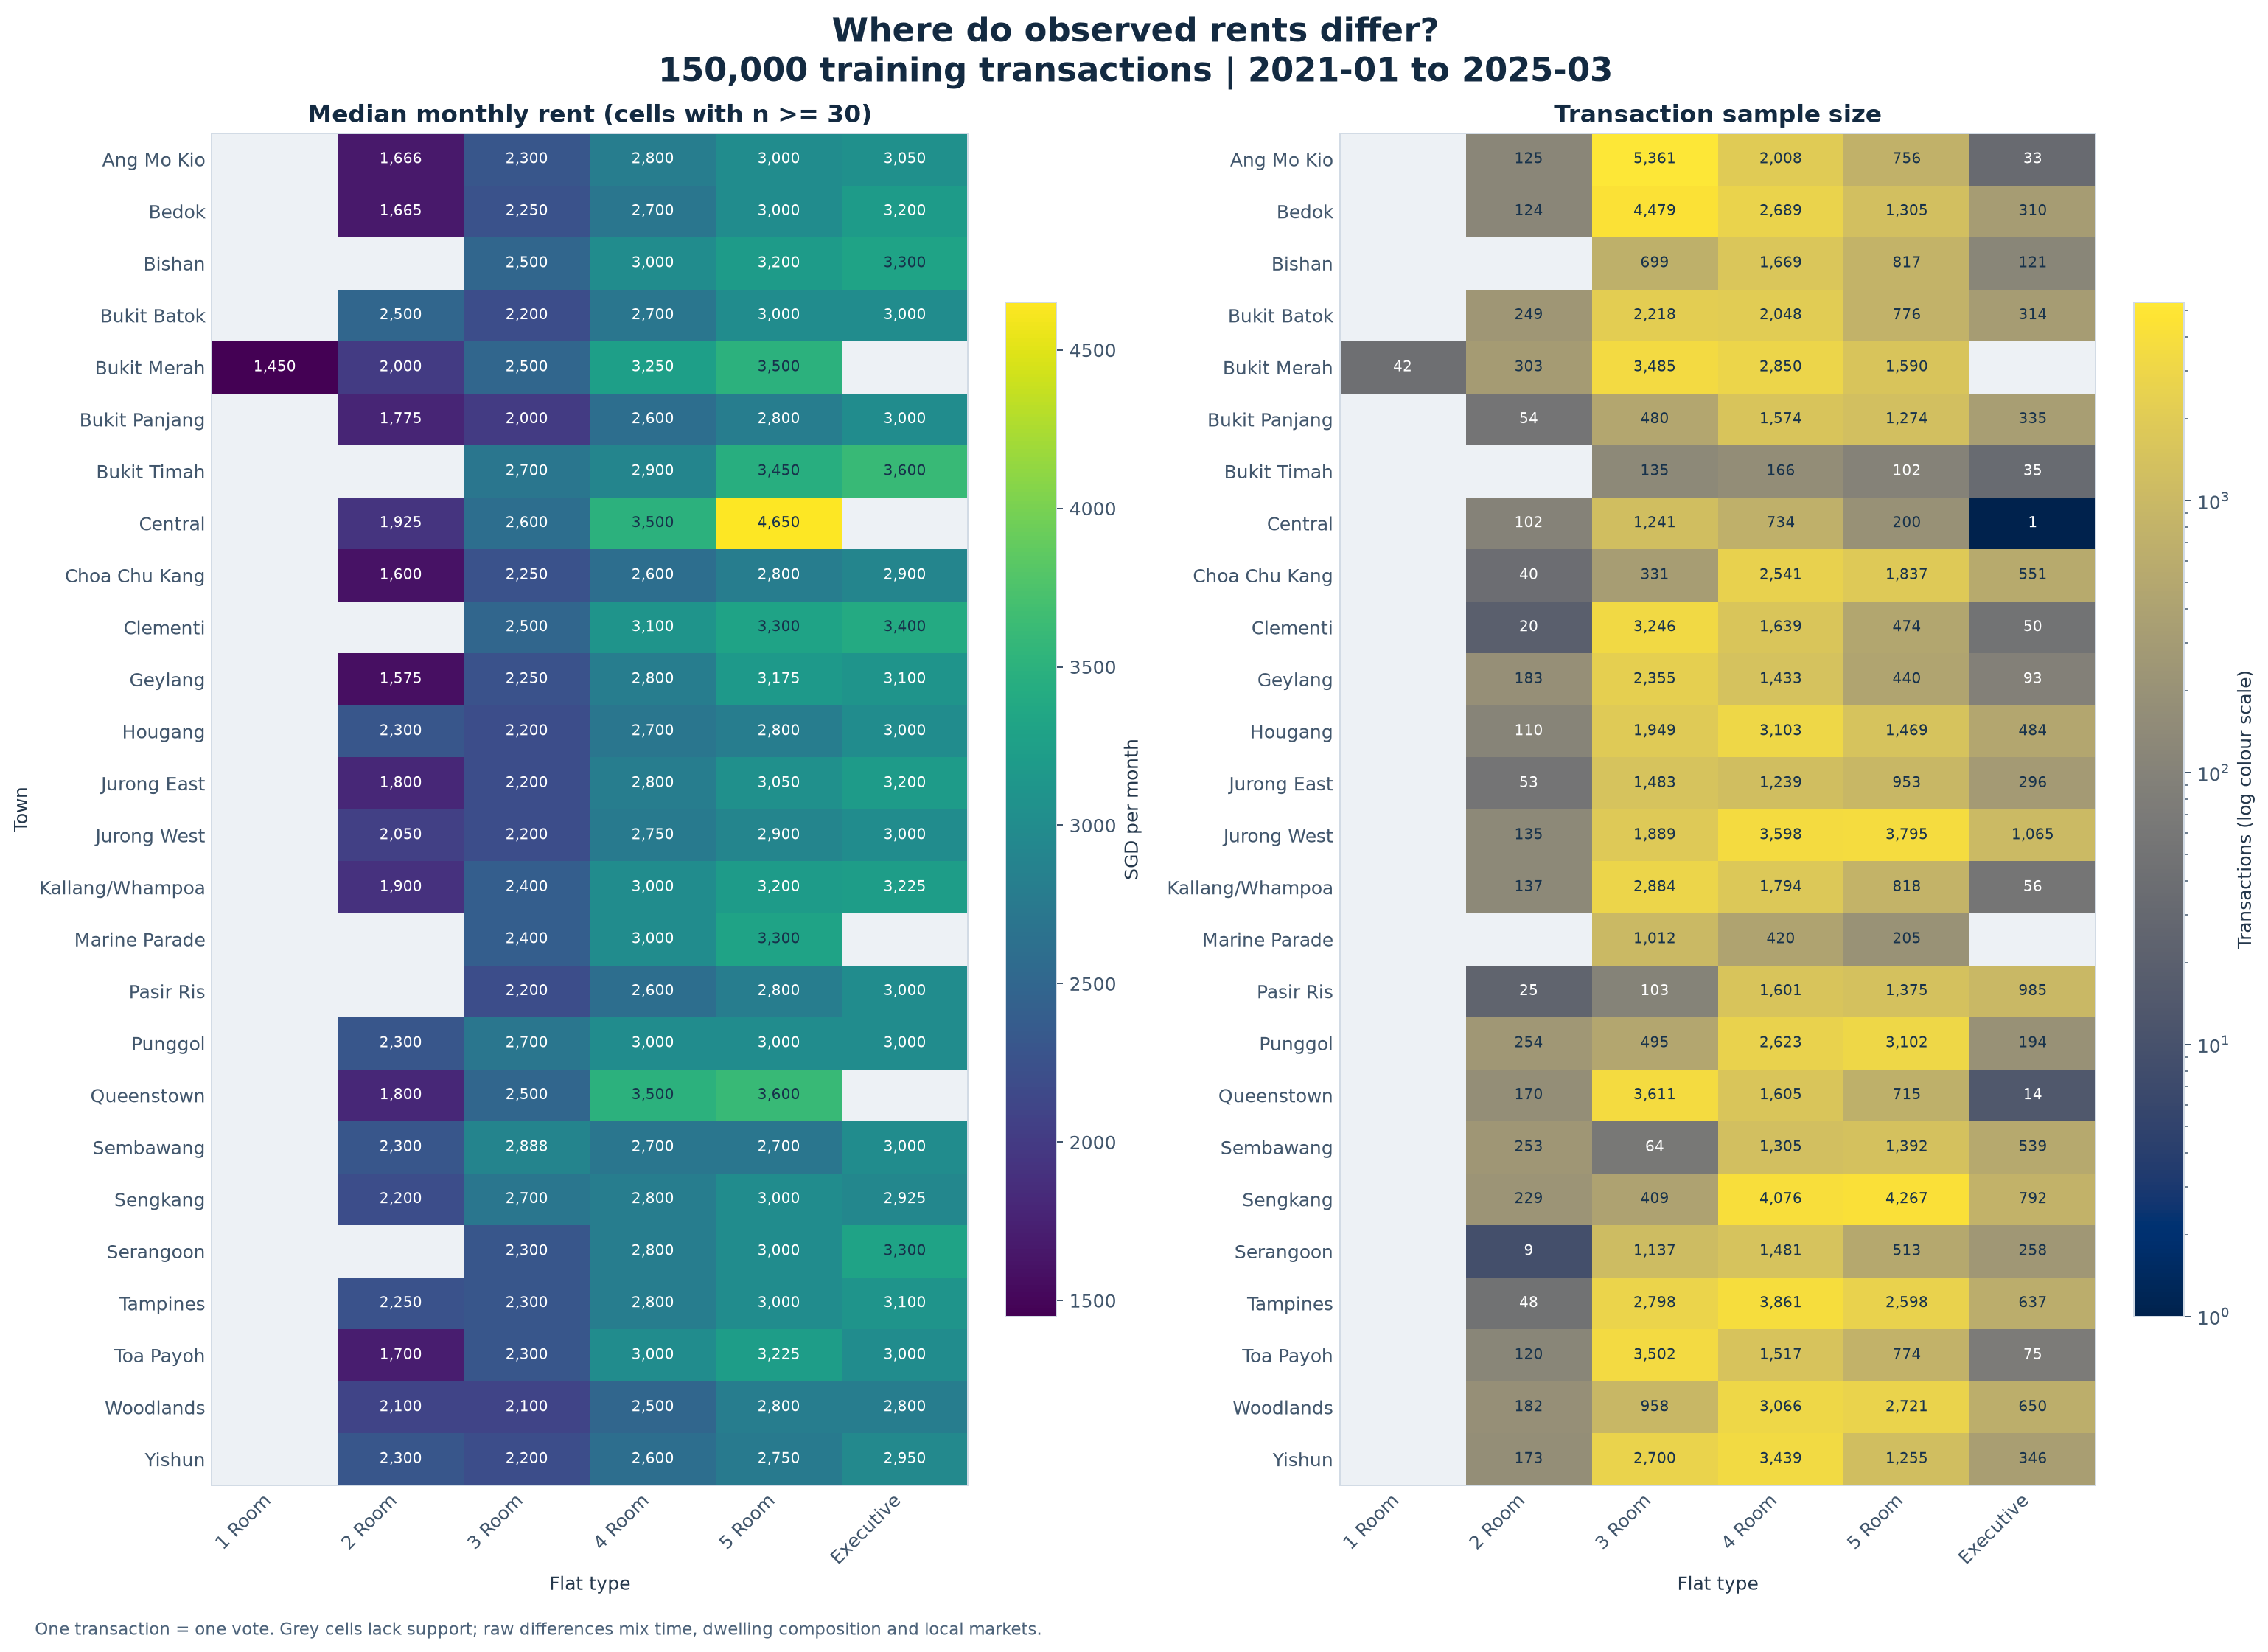
\includegraphics[width=0.98\linewidth,height=0.58\textheight,keepaspectratio]{distribution_01_town_flat.png}
\caption{Town by flat type: median observed rent and sample count.}
\label{fig:townflat}
\end{figure}

Figure~\ref{fig:monthtown} contrasts the raw monthly median rent with a mean residual from a descriptive ridge fit on the labelled rentals.
The ridge uses area, log area, flat type, flat model, and town, and it does not use month.
The residual is observed rent minus fitted rent, in SGD.
The fit uses the labelled months through March 2025, so it is not a training-set-only fit and it is not an out-of-sample error.

\begin{figure}[htbp]
\centering
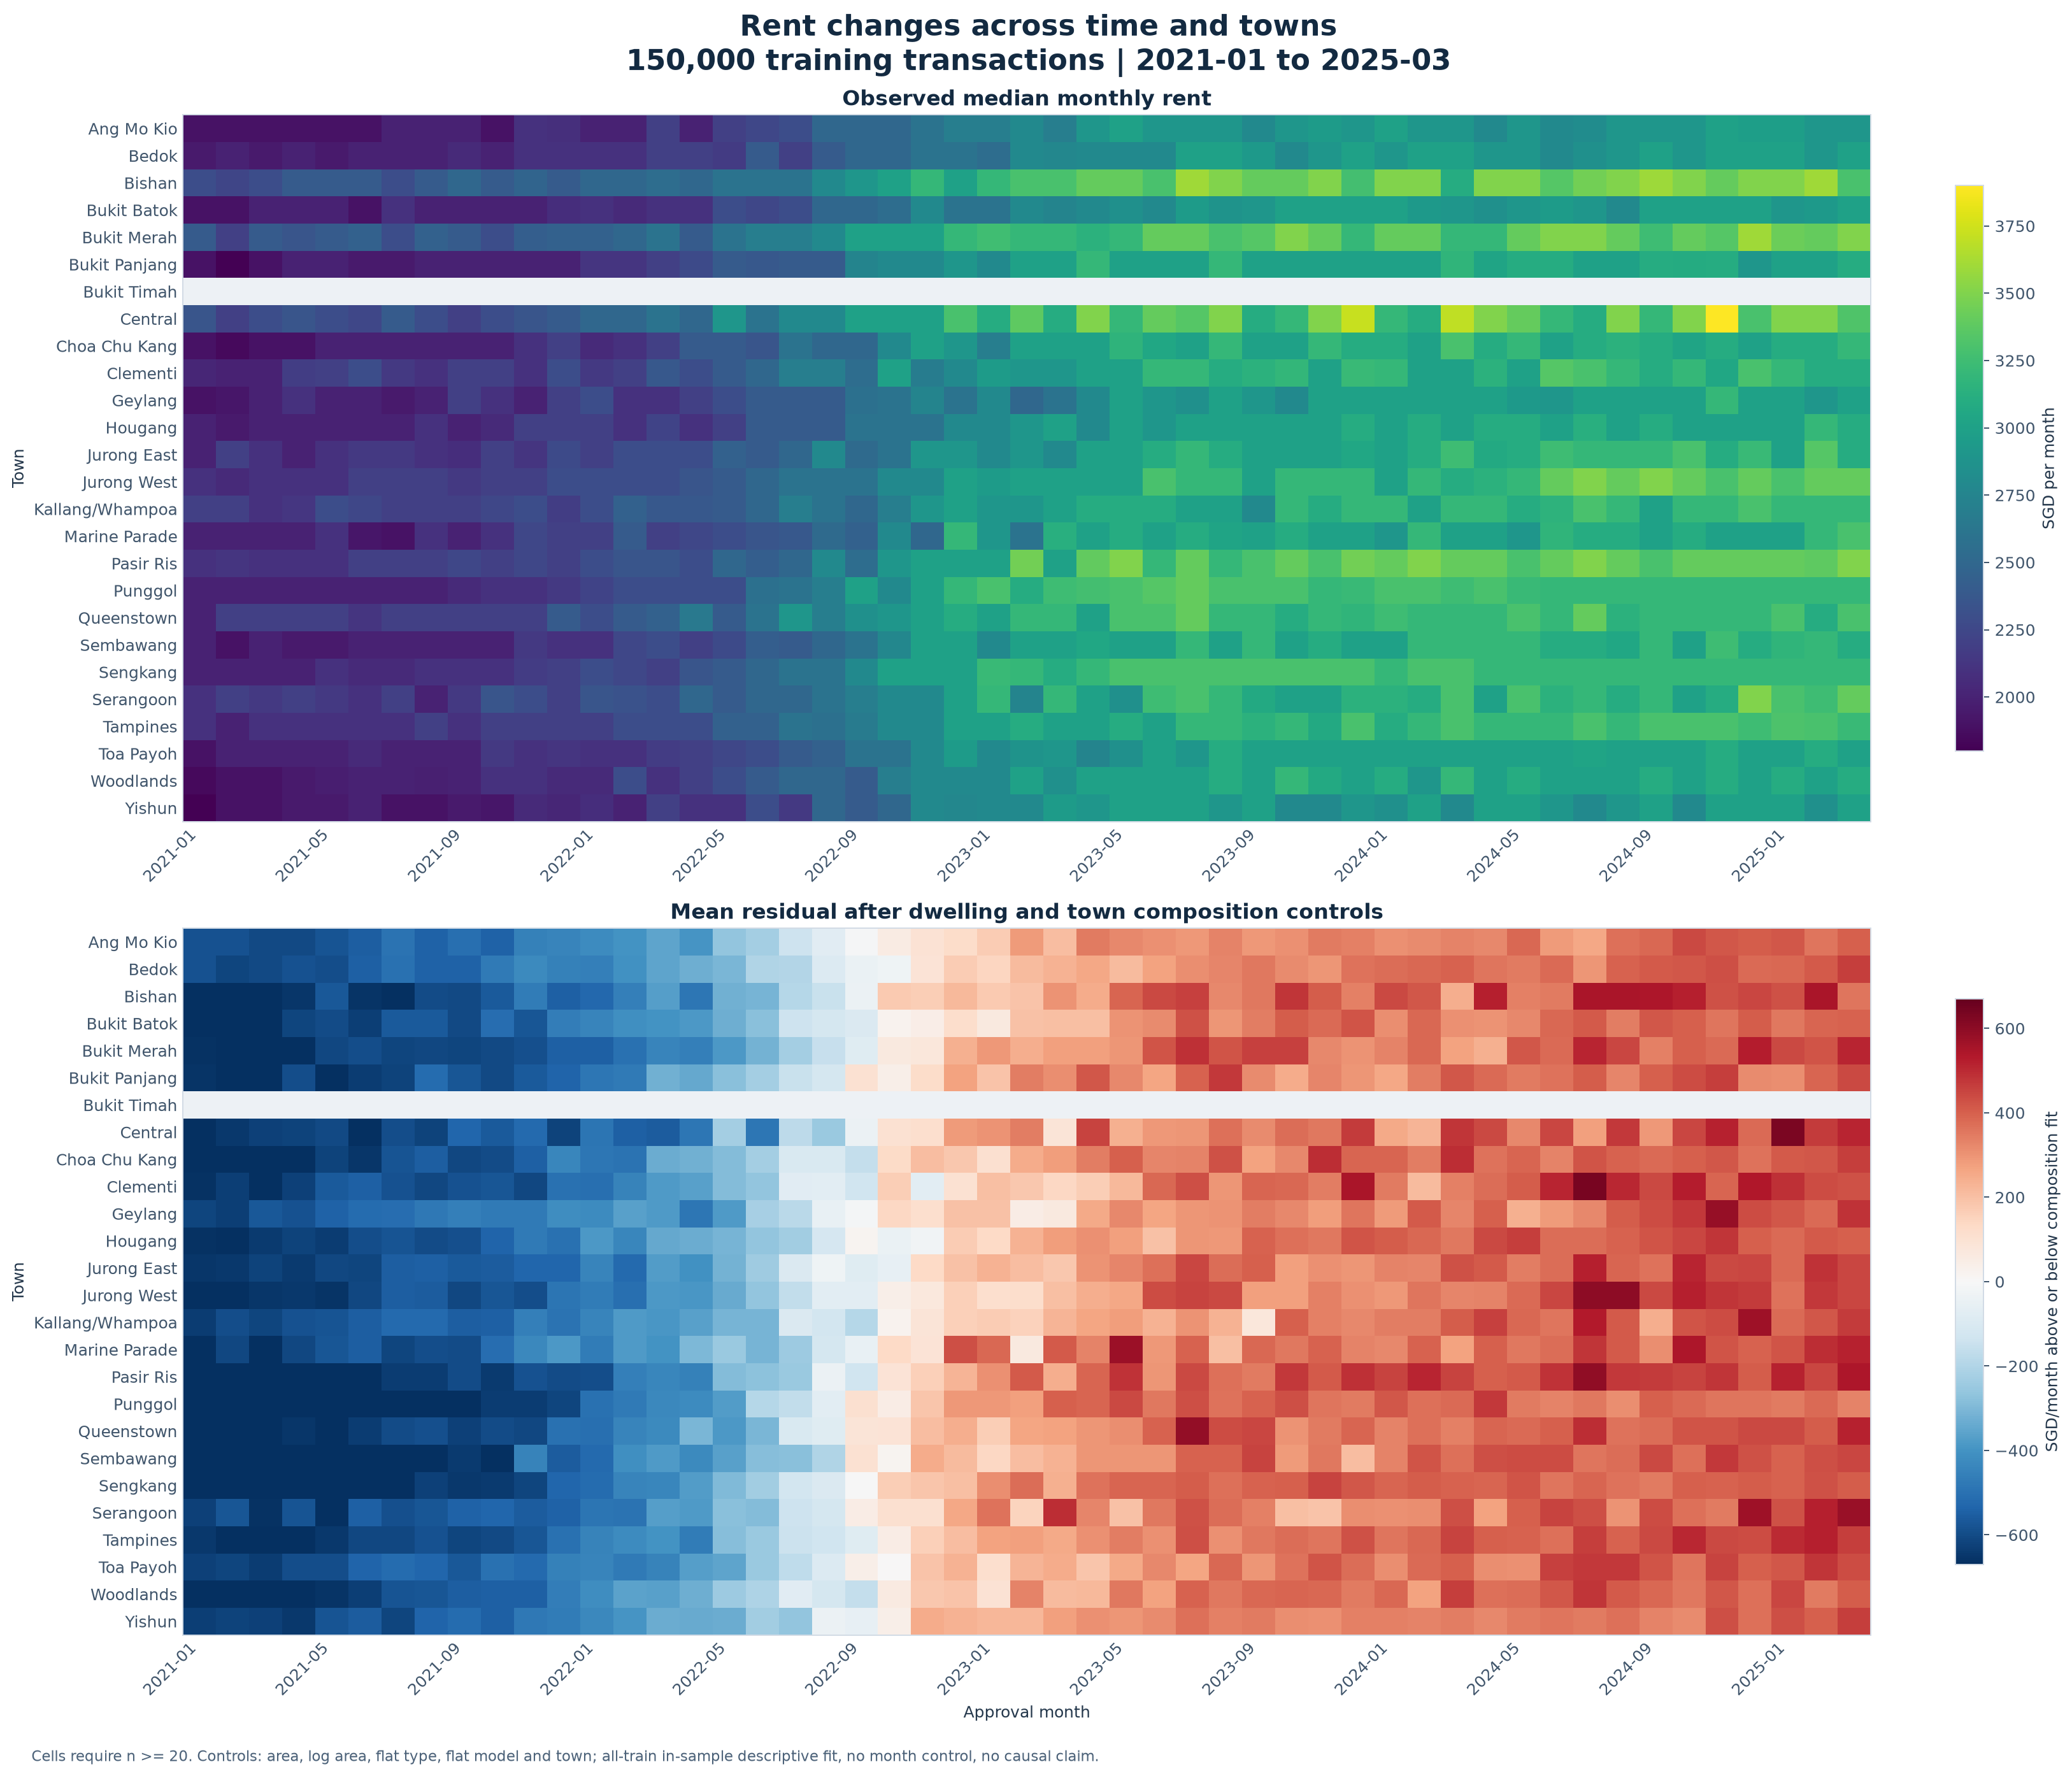
\includegraphics[width=0.98\linewidth,height=0.58\textheight,keepaspectratio]{distribution_02_month_town.png}
\caption{Monthly town distributions: raw rent and composition-adjusted residuals, with sample coverage.
The residual is descriptive.}
\label{fig:monthtown}
\end{figure}

The geographic display uses 8{,}134 blocks with at least five observed rentals.
Each block contributes one plotted rent-per-area summary.
The middle panel of Figure~\ref{fig:geo} counts distinct observed blocks in each spatial cell.

\begin{figure}[htbp]
\centering
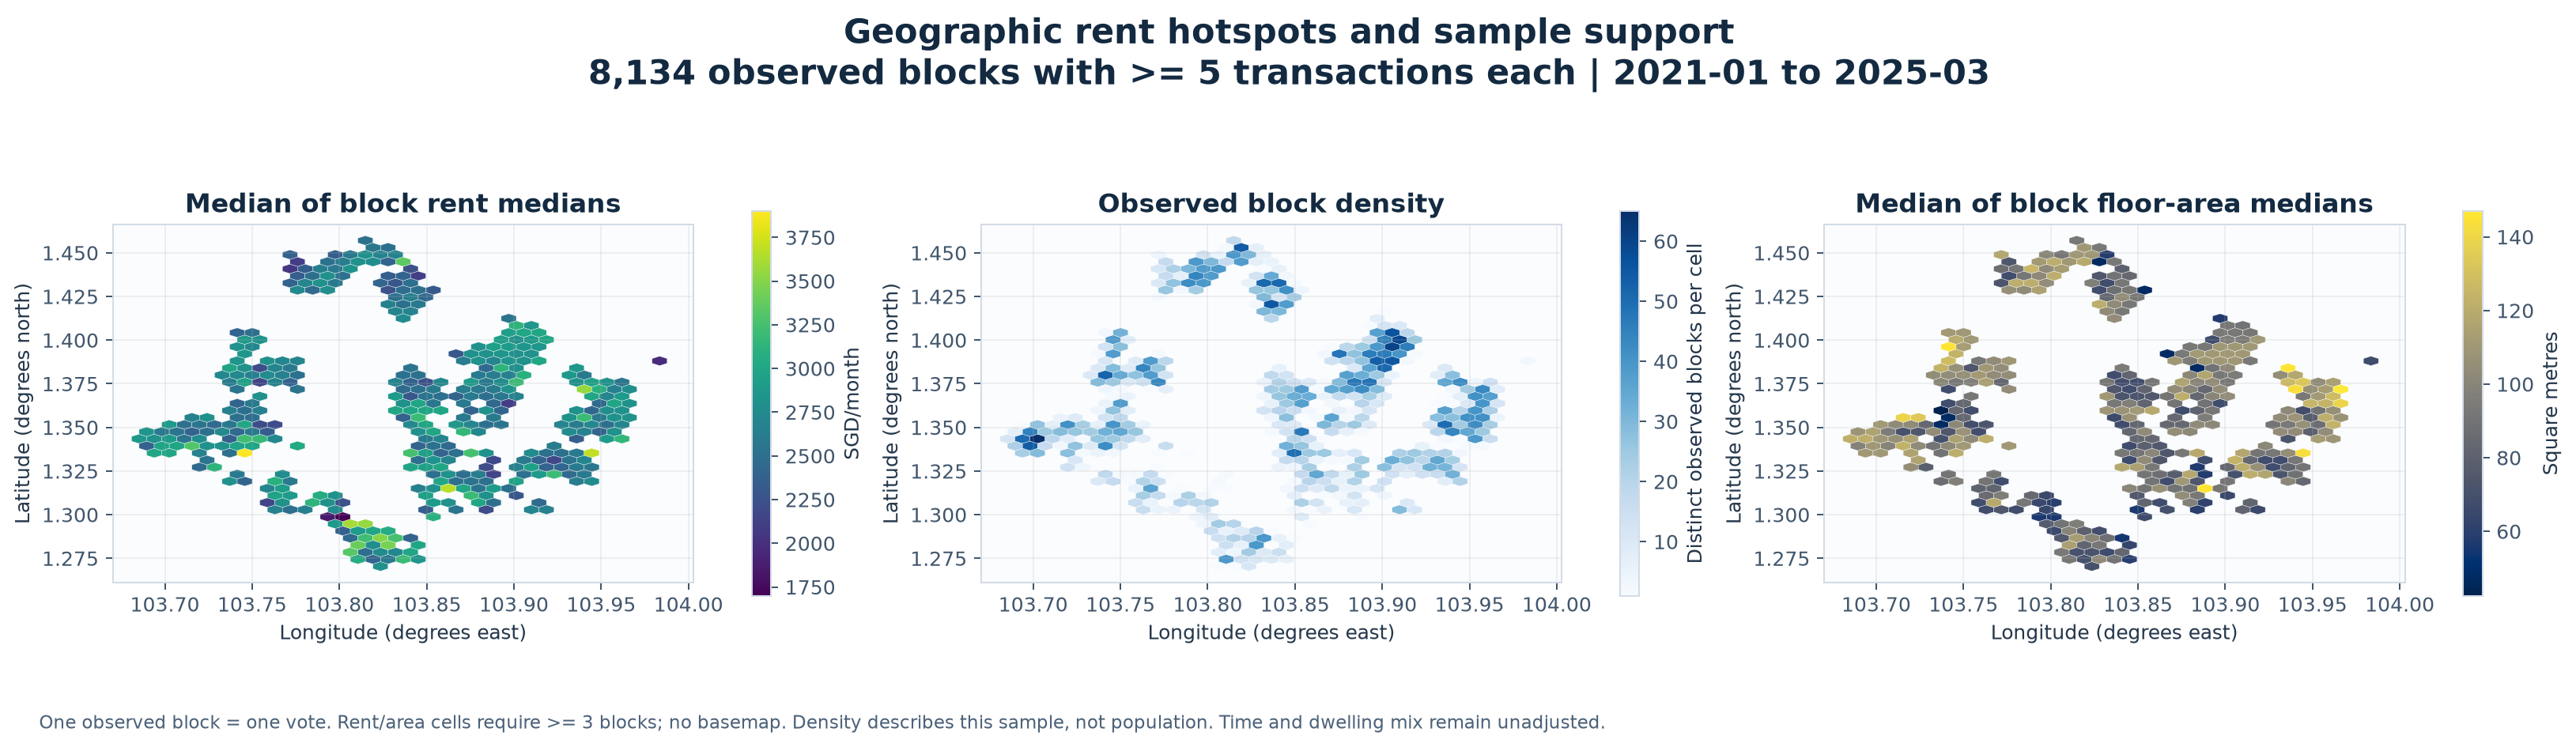
\includegraphics[width=0.98\linewidth,height=0.56\textheight,keepaspectratio]{distribution_03_geo_hotspots.png}
\caption{Block-level rent, counts of distinct observed blocks per spatial cell, and area.}
\label{fig:geo}
\end{figure}

Figure~\ref{fig:dwelling} is the original dwelling panel.
It compares area and lease-age bands by flat type, and it places flat-model median rent beside the sample count.
Cells with fewer than 50 observations are masked, and their counts remain visible.
The panel uses the labelled rentals from January 2021 through March 2025.
Larger area, flat type, lease cohort, and flat model have to be read together with geography and month.
They are not isolated causal premiums.

\begin{figure}[htbp]
\centering
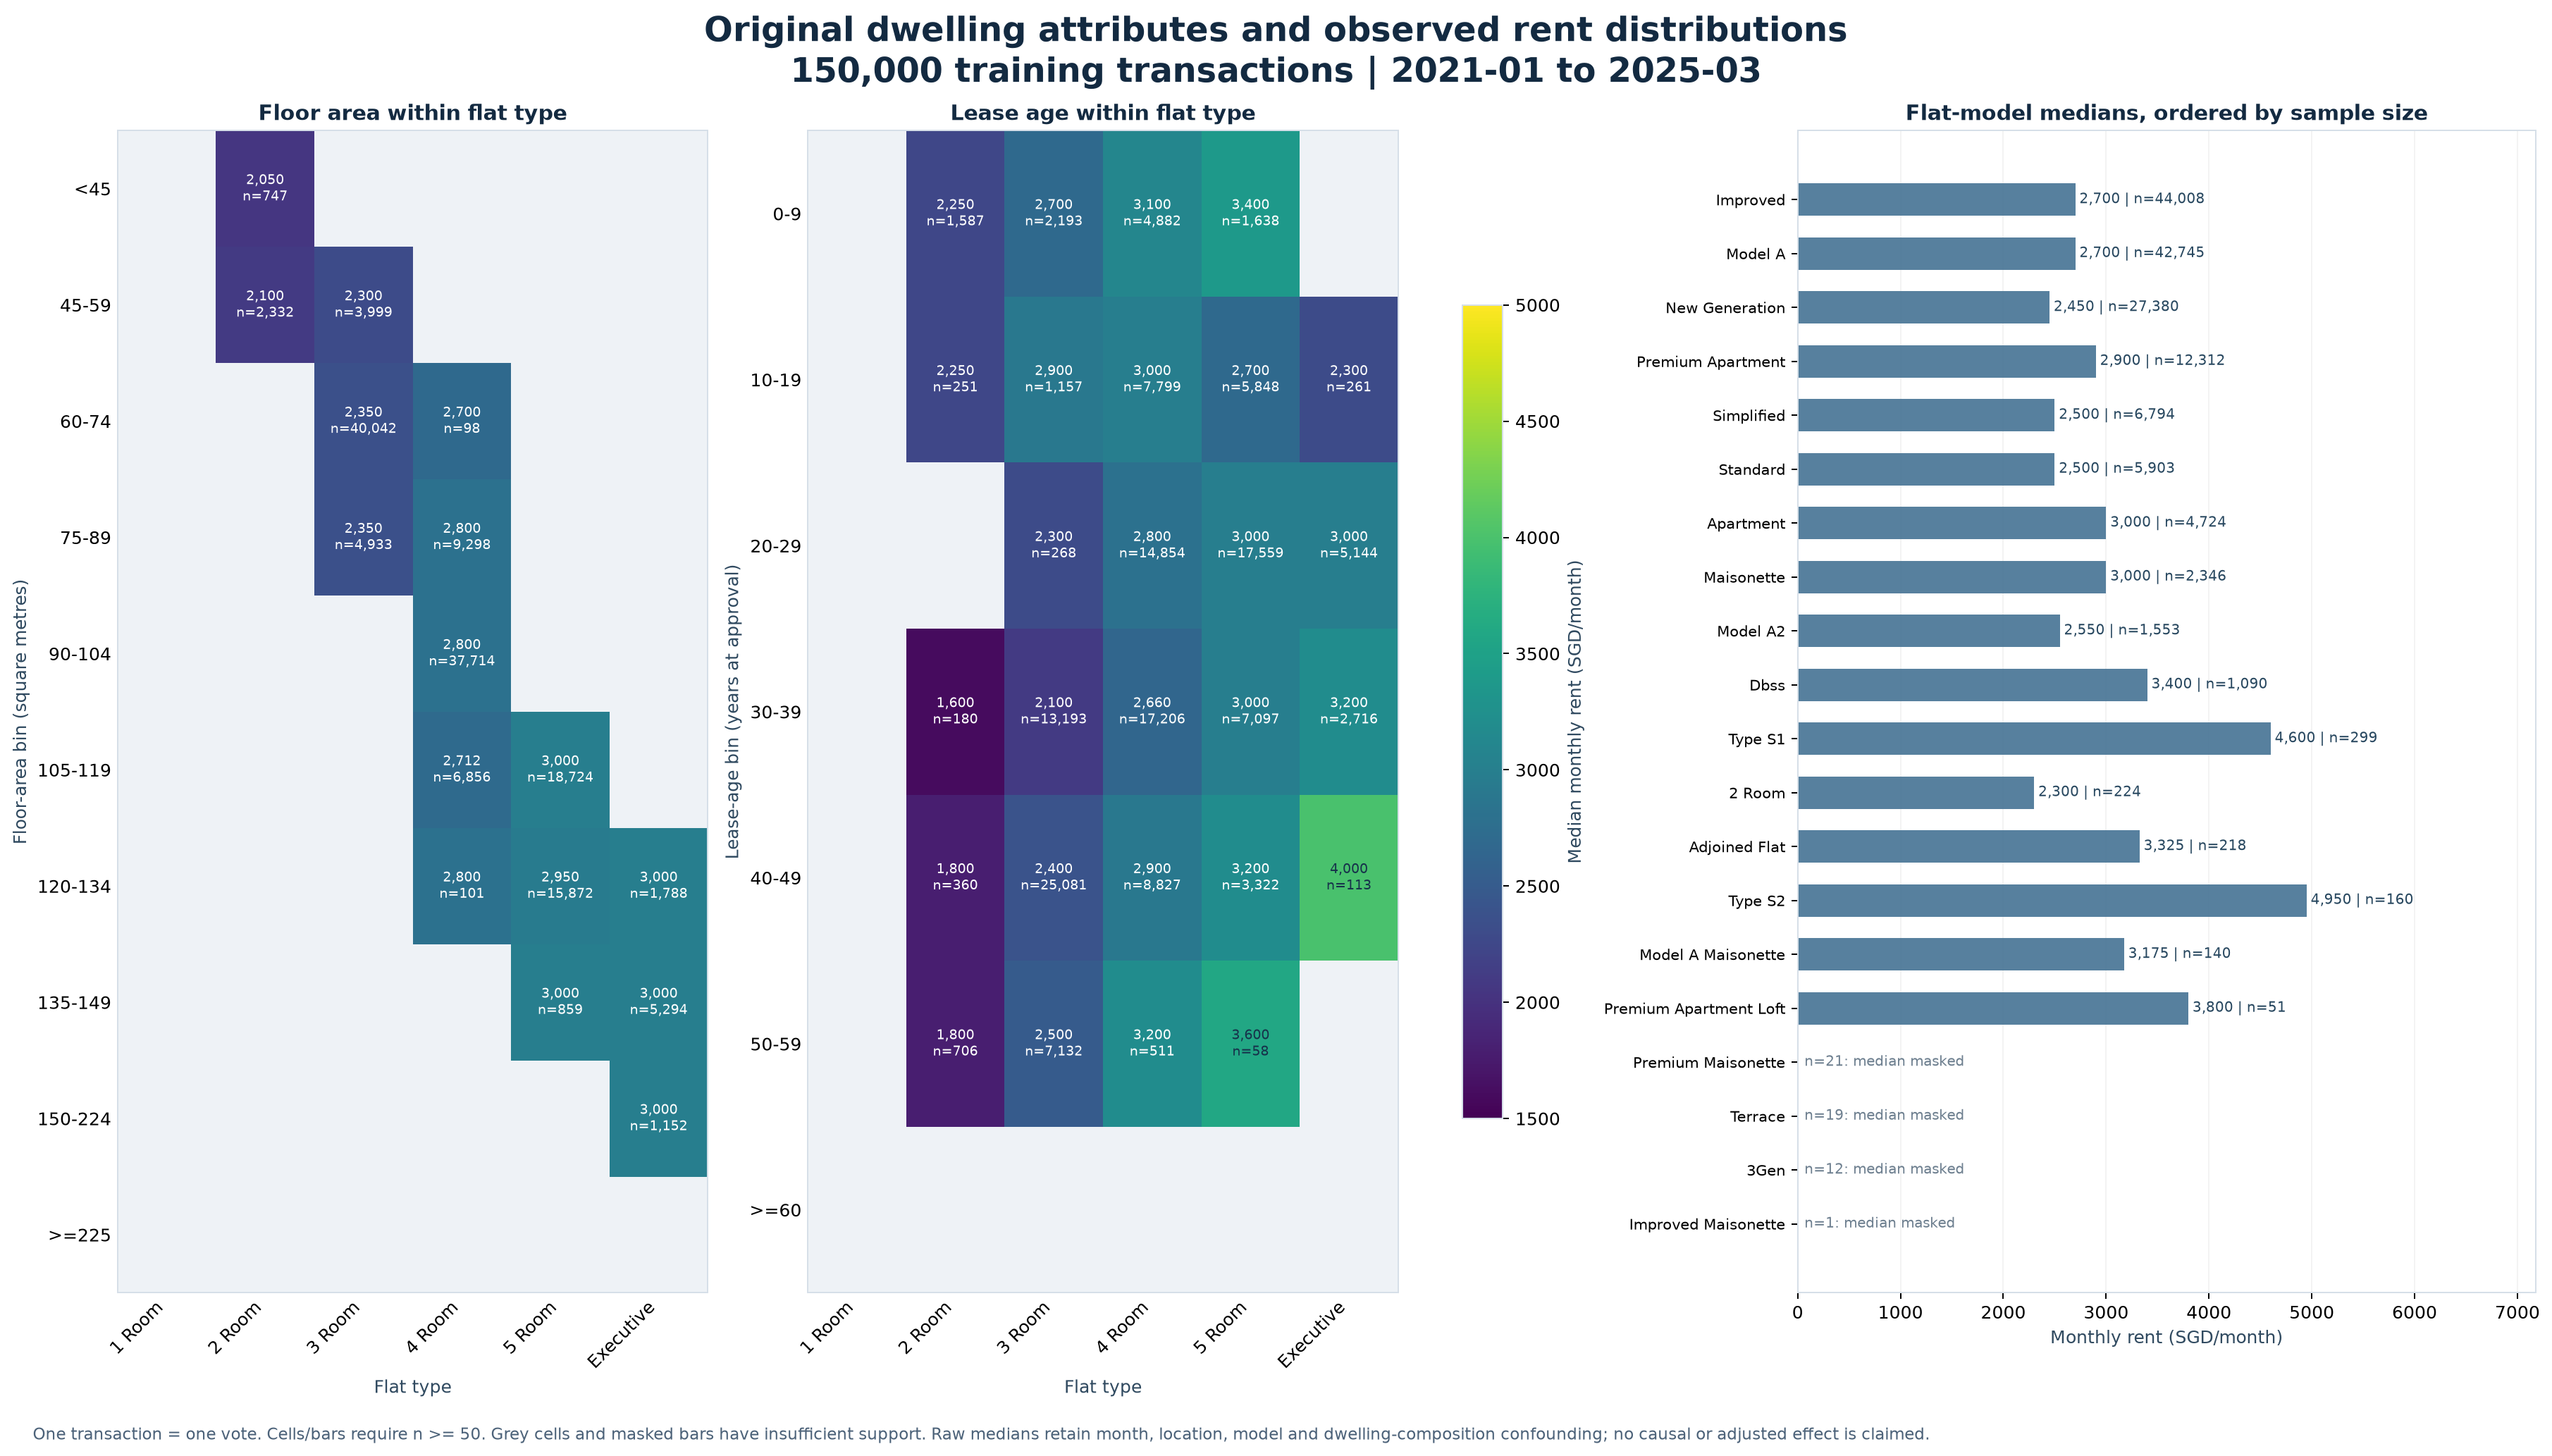
\includegraphics[width=0.98\linewidth,height=0.52\textheight,keepaspectratio]{distribution_07_original_dwelling.png}
\caption{Original dwelling attributes on the labelled rentals.
Cells with fewer than 50 observations are masked.
The panel is descriptive.}
\label{fig:dwelling}
\end{figure}

\FloatBarrier
\section{Features preprocessing: core rental fields}
\label{sec:core}

The raw labelled table and the private test set are left unchanged.
Cleaning is applied afterwards, with the same functions on both files, so that a category has one representation.
No row is removed unless there is clear evidence that it is invalid.
At the end of this stage, none has been removed.
Duplicate transactions and unusual rents stay in the data.

\subsection{Categorical fields}

The fields for town, block, street, flat type, flat model, and furnished status are stripped, lower-cased, and reduced to a single internal space.
Street names are the largest inconsistency.
The labelled data contain 1{,}146 raw street labels and 576 values after case and whitespace normalization.
The unlabelled file falls from 1{,}129 raw labels to 573 normalized street names.
The change rewrites 30{,}781 labelled rows and 10{,}482 unlabelled rows.
It does not change the street those rows name.

Flat type has a second inconsistency: \texttt{4 room} and \texttt{4-room} name the same flat.
One- to five-room labels are standardized to the hyphenated form by a deterministic rule.
That reduces the labelled categories from 11 to 6 and modifies 35{,}331 labelled rows.
The unlabelled file already uses the standardized names, so none of its rows change.
Table~\ref{tab:category-cleaning} records the two main rewrites.

\begin{table}[htbp]
\centering
\caption{Categorical standardization of the core fields.}
\label{tab:category-cleaning}
\small
\begin{tabular}{lrrrr}
\toprule
Feature & Labelled before & Labelled after & Labelled rows changed & Unlabelled rows changed \\
\midrule
Street & 1{,}146 & 576 & 30{,}781 & 10{,}482 \\
Flat type & 11 & 6 & 35{,}331 & 0 \\
\bottomrule
\end{tabular}
\end{table}

Furnished status and the upfront fee are constant.
Furnished status is yes on every labelled row and every row of the private test set.
The fee is 0 on every row.
Neither field varies.
Both are removed from the cleaned modelling table used for the core baselines.

\subsection{Time, building, and lease age}

Approval dates are parsed into a year, a calendar month, and a month index.
January 2021 has month index 0:
\begin{equation}
\label{eq:month-index}
\mathrm{month\ index}
=
12(\mathrm{approval\ year}-2021)
+
(\mathrm{approval\ month}-1).
\end{equation}
Labelled values run from 0 to 50.
The private test set continues to 66, which is July 2026.
September 2024 is 44.
The index keeps chronological order.
The year and the calendar month are kept as well, because a single continuous index does not by itself represent a within-year pattern.

A building identifier concatenates the normalized block and the normalized street.
Block number alone is ambiguous, because the same number occurs on different streets.
The labelled data have 9{,}406 buildings, and the unlabelled file has 8{,}940.

Lease age is the approval year minus the lease commencement year, so the same commencement year is a different age in 2021 and in 2025.
One labelled row has a commencement year later than its approval year.
That row is kept.
An indicator is set, and only the derived lease age is stored as null.
The private test set has no such row.
After the derived time fields exist, the original approval-date string is dropped.
Table~\ref{tab:derived-core-features} lists the derived core fields.

\begin{table}[htbp]
\centering
\caption{Fields derived from the core rental columns.}
\label{tab:derived-core-features}
\small
\begin{tabular}{lll}
\toprule
Derived field & Source & Role \\
\midrule
Approval year & approval date & long-run level \\
Approval month & approval date & calendar month \\
Month index & year and month & chronological order \\
Building & block and street & street-specific block \\
Lease age & approval year and lease year & age at approval \\
Invalid lease age & the one reversed pair & keep the row, null the age \\
\bottomrule
\end{tabular}
\end{table}

\subsection{Ranks and keys used by the multistage model}
\label{sec:ranks}

The core baselines use the cleaned categories directly.
The multistage model also uses a small set of derived keys and ranks.
None of them reads monthly rent in order to build the flat-type rank.
The same maps are applied to the labelled rows and to the private test set.

The flat-type rank turns hyphens into spaces and maps 1-room through 5-room to 1 through 5 and executive to 6.
Median floor area rises along that order, from about 31 square metres for a 1-room flat to about 144 for an executive flat.
The rank is that size order.
The flat-model rank is a fixed order from 0 through 19, from cheaper to dearer names in the labelled table.
A separate key keeps the normalized flat-model name, so a tree can split on a subset of names.
The mixture and the numeric network receive only the rank.
The labelled table has 20 flat-model names.
The private test set has 19 of them, and it has no name that is absent from the labelled table.

Town, block, and street keys strip, lower-case, and collapse spaces.
They are names, not price ranks.
The stored block key is the normalized block token only, and letters inside the block token are kept.
The block-and-street string used to join the block file is a separate key.
It is the building identifier above, and it is not stored as the block key.
Lease commencement year stays a four-digit year and is not rewritten as a month index.
Floor area and the fee amount stay in the units as recorded.
They are not standardized on the combined labelled and unlabelled tables.

\subsection{Duplicates, anomalies, and coverage}

Duplicate rows are inspected and kept.
The table records transactions, so two rows can share an approval month, a building, a flat type, and an area and still be distinct leases.
The same predictors can also sit beside different rents, because the files do not record every tenancy-specific fact.
Every unlabelled row needs one prediction and has to stay in its original position.
Deleting a duplicate unlabelled row would break that alignment.

Floor area is checked for non-positive or implausible values, lease commencement is compared with the approval year, and labelled rents are checked for non-positive values.
These checks mark rows for inspection.
They are not deletion rules.
A large or small rent is not treated as an error merely because it falls outside a generic interquartile fence.
Housing rents vary with location, flat type, age, and time.
A peer-rent diagnostic, when used, is computed after a chronological split and from the fitting portion's labels only.
It is not an input feature, and no row is removed on the basis of it.

After normalization, the unlabelled file introduces no new value of town, street, flat type, or flat model.
Eleven block labels are new, on 36 rows, and 50 building identifiers are new, on 102 rows.
That is about 0.07\% of unlabelled rows for a new block label and about 0.20\% for a new building.
The encoder has to accept an unseen category, and the mismatch is limited.
Town and street still identify the flat when the building itself is new.
Table~\ref{tab:train-test-category-coverage} is the coverage count.

\begin{table}[htbp]
\centering
\caption{Categorical coverage after normalization.
``Unseen'' means a value present in the unlabelled file and absent from the labelled table.}
\label{tab:train-test-category-coverage}
\small
\setlength{\tabcolsep}{4pt}
\begin{tabular}{lrrrr}
\toprule
Feature & Labelled unique & Unlabelled unique & Unseen values & Unlabelled rows \\
\midrule
Town & 26 & 26 & 0 & 0 \\
Street & 576 & 573 & 0 & 0 \\
Flat type & 6 & 6 & 0 & 0 \\
Flat model & 20 & 19 & 0 & 0 \\
Block & 2{,}720 & 2{,}660 & 11 & 36 \\
Building & 9{,}406 & 8{,}940 & 50 & 102 \\
\bottomrule
\end{tabular}
\end{table}

\subsection{What may be learned before a split}

Deterministic steps may be applied before any chronological split.
Those steps are text normalization, flat-type standardization, date parsing, and the construction of the building identifier and lease age.
Anything estimated from the data is fit on the fitting portion of that experiment only.
Table~\ref{tab:preprocessing-leakage} is the rule.
It matters most for high-cardinality fields such as building, block, and street: if a later encoding uses rents, rents from the scored months of that experiment do not enter the encoding.
The windows themselves are defined in Section~\ref{sec:models}.
This table does not rename them.

\begin{table}[htbp]
\centering
\caption{Which preprocessing steps may precede a chronological split.}
\label{tab:preprocessing-leakage}
\small
\begin{tabular}{lll}
\toprule
Operation & Before the split? & Rule \\
\midrule
Text normalization & Yes & deterministic \\
Flat-type standardization & Yes & deterministic \\
Date parsing & Yes & deterministic \\
Building and lease age & Yes & deterministic \\
Missing-value imputation & No & fitting portion only \\
Feature scaling & No & fitting portion only \\
Target encoding & No & fitting labels only \\
Historical mean rent & No & earlier fitting rows only \\
Target-based outlier statistics & No & fitting portion only \\
\bottomrule
\end{tabular}
\end{table}

The cleaned files keep a log of the issue, the rule, the reason, and the number of affected rows.
The private-test row order is preserved.
The next stage attaches block, transport, amenity, and market columns without changing that order.

\FloatBarrier
\section{Auxiliary features preprocessing}
\label{sec:aux}

Stations, schools, and malls have coordinates and no block number.
The block table is the hub: it has an address and coordinates, and every later spatial column starts from that join.
Saved auxiliary tables contain the new columns in source-row order.
The original rental fields are concatenated back when a model is fit.
Labelled rows and the private test set are joined by that order, and they are not sorted.

Two ledgers appear in the work, and they are not the same column list.
The multistage model reads an auxiliary table of 94 columns in that row order.
The rebuilt audit is a larger candidate ledger.
It is the source of the locked CatBoost comparisons in Section~\ref{sec:models}.
A count from one ledger is not the width of the other.

\subsection{The rebuilt candidate audit}
\label{sec:rebuild}

The rebuilt audit reconstructs candidates from the original rental inputs and from every field in the six supplied auxiliary files.
The source ledger has 63 input-field positions: ten original rental fields and 53 auxiliary fields.
The target is recorded separately.
Furnished status and the fee are ignored, including derived indicators and interactions, which leaves 61 source positions for predictors, construction, joins, or metadata.
Source names, URLs, and keys receive explicit roles.
They are not labelled as causal rent factors.

The audit records 1{,}878 conceptual candidates, including 1{,}595 month-panel candidates.
The compact rental table stores 492 candidate columns plus row, month, target, and provenance metadata.
Individual-stock and adjusted-price candidates stay in the monthly panel and are reduced with training-month preprocessing, so the same macro vector is not copied onto every rental as if it were a flat-level measurement.
The family ledger is a candidate universe, not the dimension of a fitted model.
Table~\ref{tab:families} counts the families.

\begin{table}[htbp]
\centering
\caption{Rebuilt candidate families.
These counts are the audit ledger, not the 94-column auxiliary table.}
\label{tab:families}
\small
\begin{tabular}{lr}
\toprule
Candidate family & Columns \\
\midrule
Block structure & 5 \\
Location & 11 \\
MRT & 122 \\
Schools & 123 \\
Malls & 8 \\
COE & 164 \\
Stocks & 1200 \\
Adjusted-price sensitivity & 231 \\
Original & 14 \\
\bottomrule
\end{tabular}
\end{table}

The normalized town, block, and street key is checked as a many-to-one link, with rental row identity and order preserved.
Block features retain latitude, longitude, postal and geographic labels, completion year, and maximum building floor.
Ages, density, and location summaries are derived.
The maximum floor is not the unit floor.
Mass Rapid Transit (MRT) construction distinguishes code rows from deduplicated entities, open and planned snapshot status, line-code prefixes, interchange descriptors, distances, and radius counts.
Schools include the observed primary, secondary, junior-college, and mixed-stage definitions, together with type, gender, session, address, and transport-text descriptors.
Malls contribute identity, nearest distances, and radius counts.
COE uses the supplied categories and rounds, with premium, prevailing premium, quota, bids, and derived differences and ratios.
Stocks audit all 77 symbols and the open, high, low, close, adjusted-close, and volume fields.
Adjusted-price descriptors are a separately labelled retrospective sensitivity.
Figure~\ref{fig:stocks} shows lagged monthly-return availability for those 77 symbols.
A month is missing when the symbol has no return from the preceding completed month.
The property basket used below is missing on early rows because one constituent starts later.

\begin{figure}[htbp]
\centering
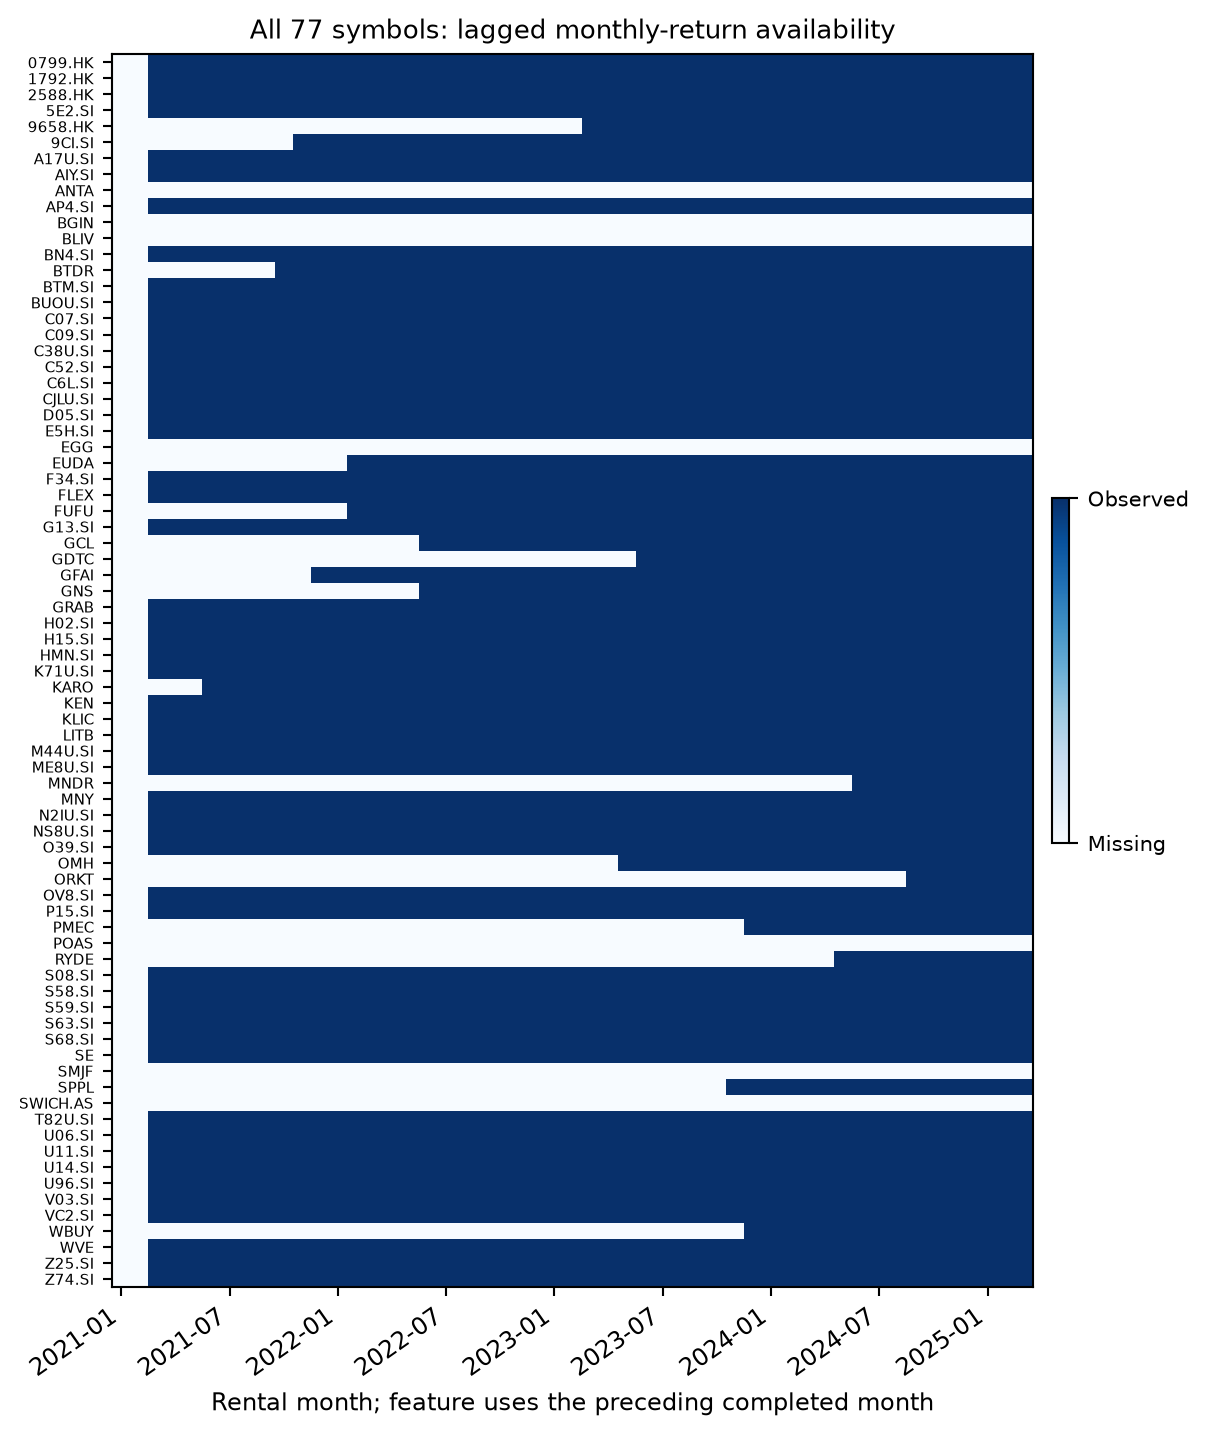
\includegraphics[width=0.86\linewidth,height=0.72\textheight,keepaspectratio]{rebuilt_all_stock_coverage.png}
\caption{Lagged monthly-return availability for all 77 audited symbols.
The property basket is missing on early rows because one constituent starts later.}
\label{fig:stocks}
\end{figure}

\subsection{Block attributes and age}

The rental row is left-joined to the block file on the normalized block concatenated with the normalized street.
Normalization strips, lower-cases, and collapses spaces, and letters inside the block token are kept.
The key matches every labelled row and every private-test row, and the row count does not change.
The copied fields are latitude, longitude, postal code, with the token \texttt{NIL} stored as null, maximum floor, year of completion, subzone, planning area, and region.
Building age is the approval year minus the completion year.
Lease age uses the lease commencement year instead.
A third column is the gap between those two ages, and a product of building age with a Central Region flag lets a linear model treat age differently in the centre.
Town alone does not say whether the block is central, new, or tall, and the same completion year is a different age in 2021 and in 2026.
Figure~\ref{fig:blocks} shows the joined region and the age and floor distributions.

\begin{figure}[htbp]
\centering
\begin{minipage}[t]{0.40\textwidth}
\centering
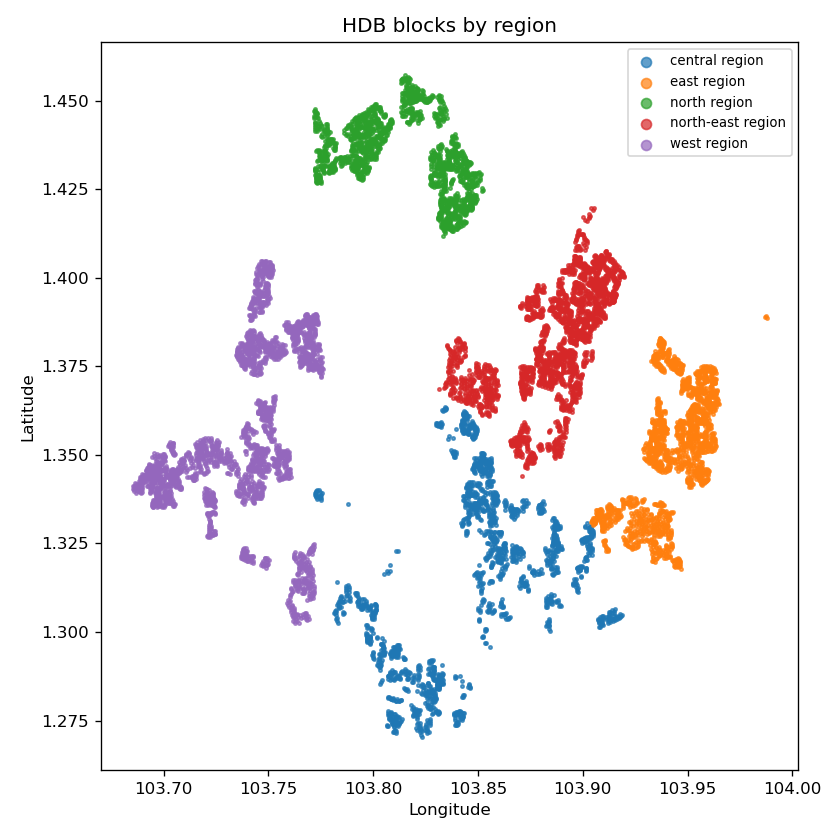
\includegraphics[width=\linewidth]{blocks_region_map.png}\\[0.35em]
{\small (a) Region after the address join.}
\end{minipage}\hfill
\begin{minipage}[t]{0.54\textwidth}
\centering
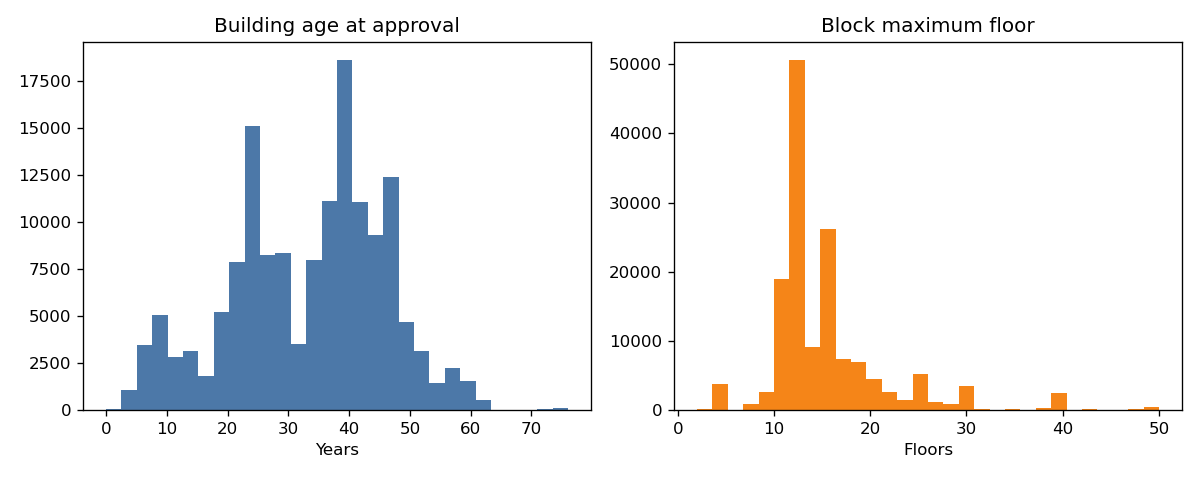
\includegraphics[width=\linewidth]{blocks_age_floor.png}\\[0.35em]
{\small (b) Age at approval, and maximum floor.}
\end{minipage}
\caption{Block attributes copied onto the rental rows.}
\label{fig:blocks}
\end{figure}

\subsection{MRT}
\label{sec:mrt}

Distances are great-circle kilometres with Earth radius 6{,}371\,km.
Two open-station pools are in the record, and they are not interchangeable.

The columns in the 94-column auxiliary table use an open trunk pool.
A station is in that pool when its status is open and its code prefix is NS, NE, CC, DT, TE, EW, or CG.
The two open Changi Airport (CG) stations are labelled EW.
For each block the table stores the nearest trunk station's distance, code, normalized name, and line, the nearest station and distance on each of the six lines, and the number of trunk codes within 0.5, 1, and 2\,km.
Ties closer than \(10^{-6}\)\,km keep the lexicographically smallest code.
Planned stations, and prefixes CR, JE, JS, JW, and CP, stay in their own distance columns, so they cannot shrink the open-station distance.
A flag is 1 when the nearest trunk station's name has at least two codes.
The reason for the split is access.
A flat near a station is easier to commute from, one distance does not say which corridor that station serves, and a count separates a single station from a cluster.
Figure~\ref{fig:mrt} shows that most rentals are within about 1\,km of some trunk station, that 0.5\,km is often empty, and that the North East Line is farther than the East--West Line.
An interchange is counted once per code.

The rebuilt audit uses a wider open-distance pool: every supplied snapshot-open station entity, which can include LRT, rather than the trunk-prefix pool.
Observed prefixes are not a verified external line taxonomy.
Station-name and line-count descriptors may combine open and planned codes at one entity, and they are read only as snapshot descriptions.
The add-MRT configuration in Section~\ref{sec:models} belongs to that rebuilt comparison.
It is not given a second definition here as the trunk-prefix columns.

\begin{figure}[htbp]
\centering
\begin{minipage}[t]{0.48\textwidth}
\centering
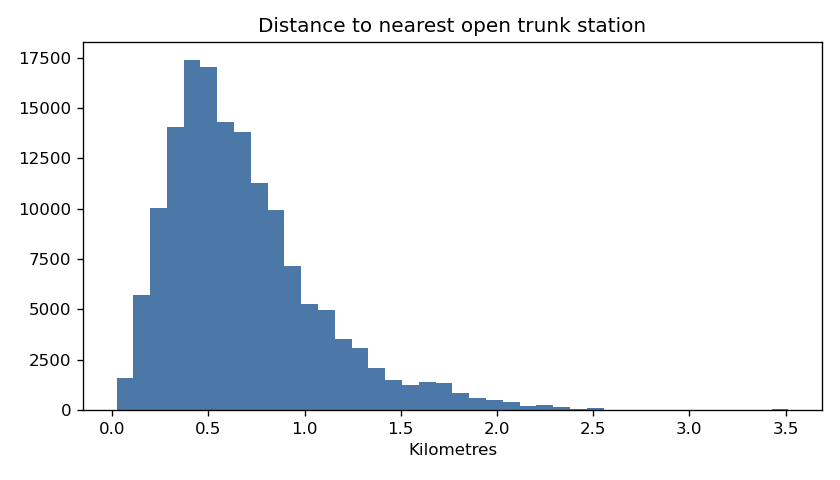
\includegraphics[width=\linewidth]{mrt_nearest_trunk.png}\\[0.3em]
{\small (a) Nearest open trunk station.}
\end{minipage}\hfill
\begin{minipage}[t]{0.48\textwidth}
\centering
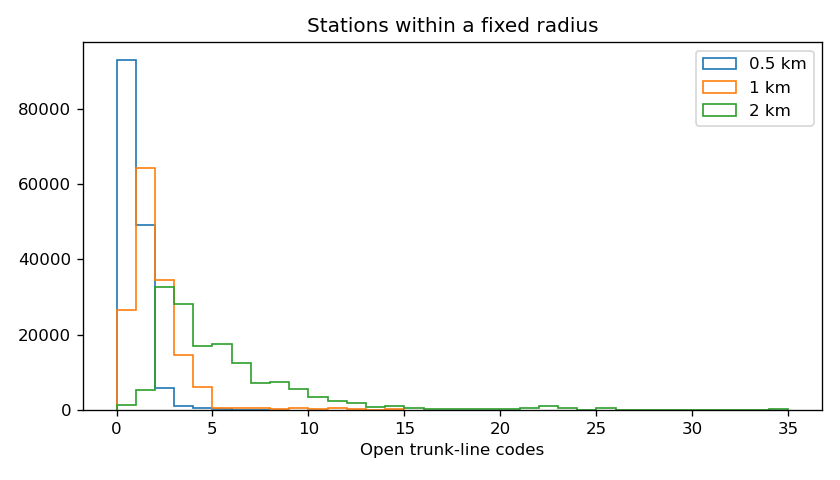
\includegraphics[width=\linewidth]{mrt_radius_counts.png}\\[0.3em]
{\small (b) Trunk-line codes within 0.5, 1, and 2\,km.}
\end{minipage}

\vspace{0.7em}
\begin{minipage}{0.62\textwidth}
\centering
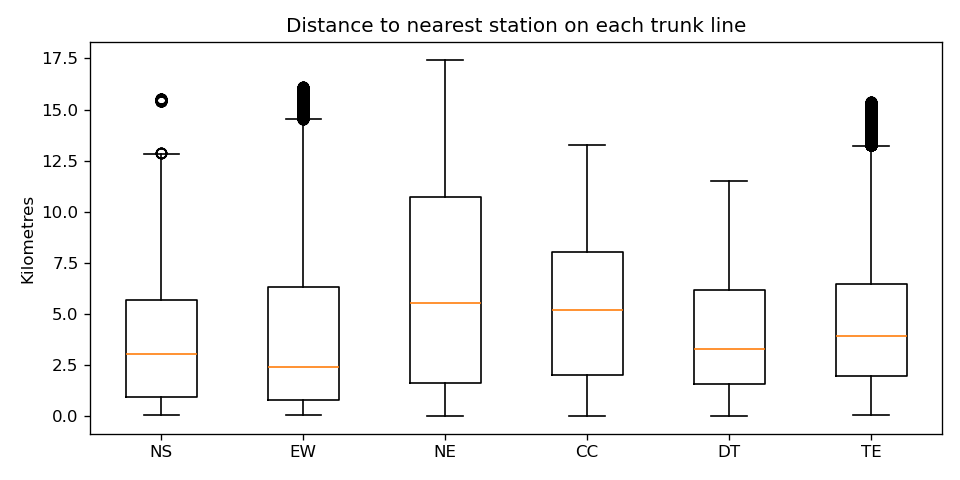
\includegraphics[width=\linewidth]{mrt_line_distances.png}\\[0.3em]
{\small (c) Nearest station on each trunk line.}
\end{minipage}
\caption{MRT access under the trunk-prefix pool.
An interchange is counted once per code.}
\label{fig:mrt}
\end{figure}

\subsection{Schools and malls}

Primary schools are rows whose main level is primary: 179 schools.
Secondary schools are the two strings for secondary years S1--S5 and S1--S4: 133 schools.
Each set contributes a nearest distance, the normalized school name, and a count within 1\,km.
Primary schools also have a 2\,km count.
All 337 schools add one further nearest distance, name, and 1\,km count.
All 113 malls contribute the nearest distance, normalized name, and counts within 1 and 2\,km.
Names are kept because those tables have no code, and the normalized name is unique.
Households pay for a short walk to a primary school or a shop, and a count distinguishes one neighbour from several.
Figure~\ref{fig:amenity} shows schools packed closer than malls, and many rentals with no mall inside 1\,km.

\begin{figure}[htbp]
\centering
\begin{minipage}[t]{0.60\textwidth}
\centering
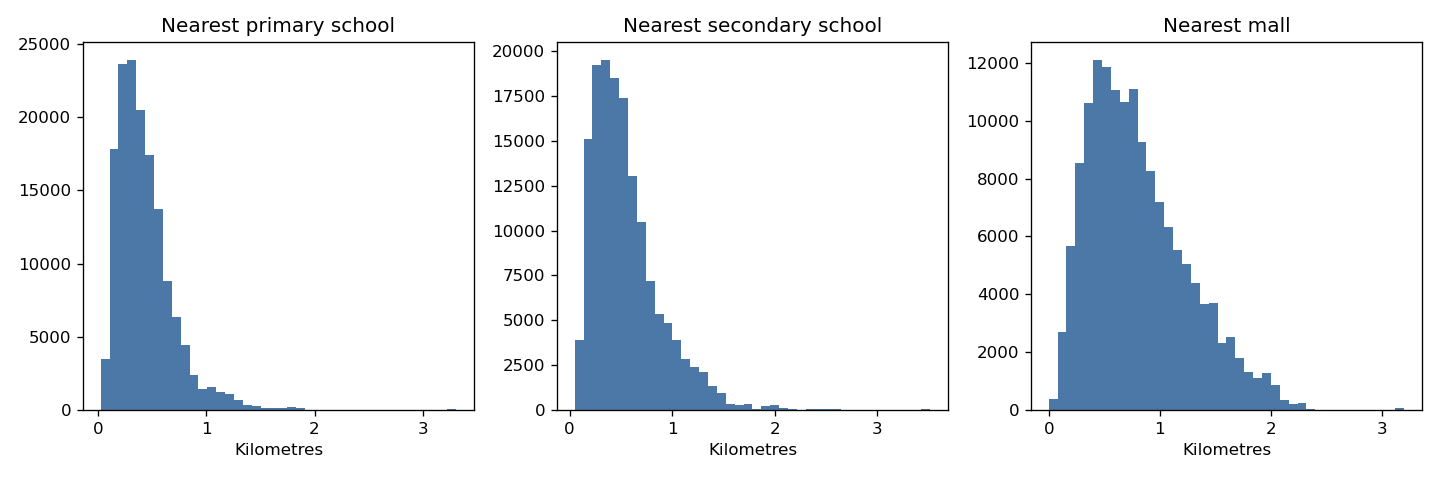
\includegraphics[width=\linewidth]{amenity_distances.png}\\[0.3em]
{\small (a) Nearest primary school, secondary school, and mall.}
\end{minipage}\hfill
\begin{minipage}[t]{0.34\textwidth}
\centering
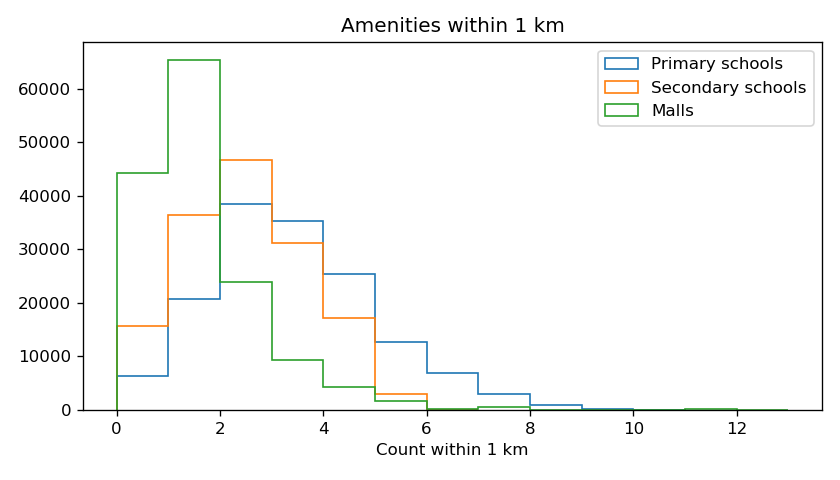
\includegraphics[width=\linewidth]{amenity_counts_1km.png}\\[0.3em]
{\small (b) Counts within 1\,km. Zero is a real zero.}
\end{minipage}
\caption{Schools and malls around the labelled rentals.}
\label{fig:amenity}
\end{figure}

\subsection{Position inside the town}

The number of other HDB blocks within 500\,m uses the same block coordinates and excludes the block itself.
The town centroid is the mean latitude and longitude of blocks in that town, and each block is measured to its own centroid.
Distance to the central business district is the great-circle distance to the fixed Raffles Place coordinate \((1.283889,\ 103.851389)\), taken from station codes \texttt{ns26} and \texttt{ew14}.
A log of the nearest trunk distance, \(\ln(d+0.001)\), gives nearby changes more weight than a linear model would give the raw kilometres.
Two flats in the same town can still sit at the edge or next to downtown.
These density columns do not use rent.
Cluster labels were not adopted.
The official areas already exist, and clustering on rent would put the target into the features.

\subsection{COE, stocks, and recent local rents}

COE amounts are parsed by stripping dollar signs and commas.
Each category-month uses bidding round 2, or round 1 when round 2 is absent.
A rental in month \(T\) receives the premium, the change from \(T-2\) to \(T-1\), and bids divided by quota, all from month \(T-1\).
Categories A, B, and E have those three columns.
Category A also has the mean of \(T-1\), \(T-2\), and \(T-3\).
Category C has only the lagged premium.
The four COE premiums are correlated about 0.93 with each other.
The region model in Section~\ref{sec:stack} therefore keeps one premium.

Stock features in this auxiliary table use month-end adjusted closes.
The bank basket is the equal-weight mean of \texttt{D05.SI}, \texttt{O39.SI}, and \texttt{U11.SI}.
The property basket is \texttt{C09.SI}, \texttt{U14.SI}, and \texttt{9CI.SI}.
A month is used only when all three symbols have a close.
The rental again sees month \(T-1\), both as a level and as that month's return.
Dearer car quotas or weaker bank shares may coincide with tighter household budgets, which floor area and town cannot express.
Figure~\ref{fig:market} shows that both series are constant across flats approved in the same month.
January 2021 COE lags are null because December 2020 is absent.

\begin{figure}[htbp]
\centering
\begin{minipage}[t]{0.48\textwidth}
\centering
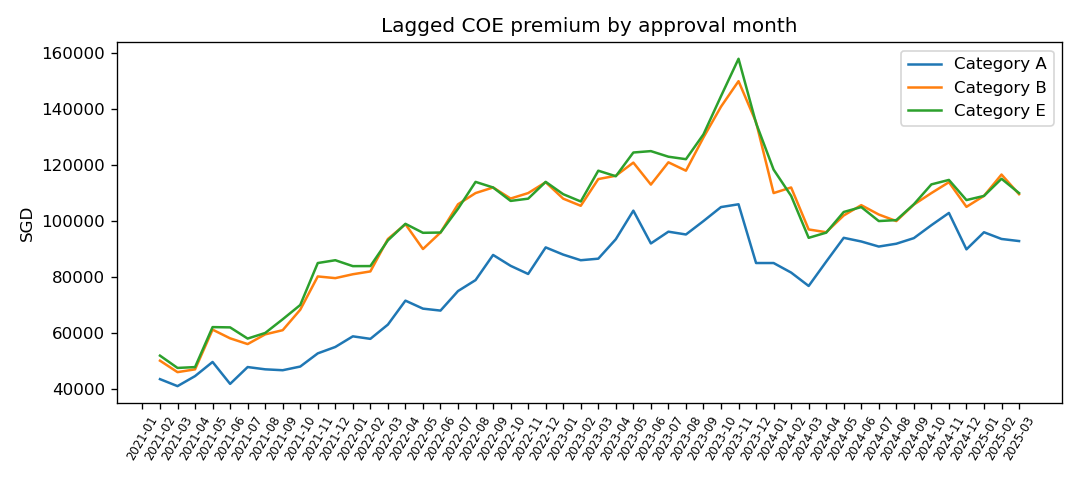
\includegraphics[width=\linewidth]{coe_monthly.png}\\[0.3em]
{\small (a) Lagged COE premium.}
\end{minipage}\hfill
\begin{minipage}[t]{0.48\textwidth}
\centering
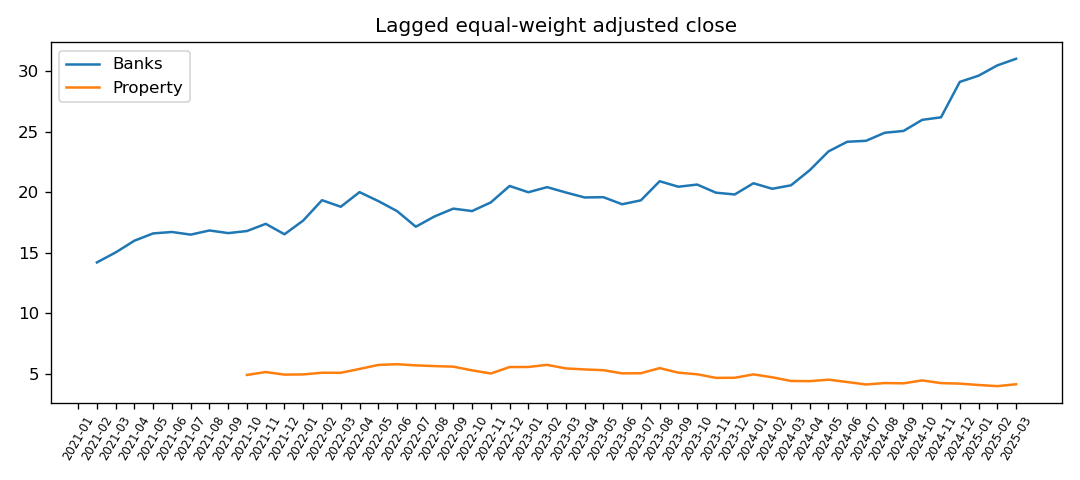
\includegraphics[width=\linewidth]{stock_baskets_monthly.png}\\[0.3em]
{\small (b) Lagged bank and property baskets.}
\end{minipage}
\caption{Month-level series shared by every flat approved in that month.}
\label{fig:market}
\end{figure}

Six columns are target encodings of recent rent.
The groups are the first two digits of the postal code, the legacy district implied by those digits, the nearest mall name, the nearest open MRT code, the nearest primary-school name, and the nearest secondary-school name.
The sector and district strings are not stored.
For a row in month \(T\), only labelled rents from \(T-1\), \(T-2\), and \(T-3\) are used:
\begin{equation}
\label{eq:shrink}
\frac{n\,\bar r_g + 20\,\bar r}{n + 20}.
\end{equation}
Here \(\bar r_g\) is the group mean inside that window, \(n\) is the number of those labelled rows, and \(\bar r\) is the island-wide mean inside the same three months.
If \(n=0\), the value is \(\bar r\).
January 2021 has none of those months in the file, so all six columns are null.
February 2021 uses January only.
Rows in the private test set never contribute rents.
The strength 20 is fixed and was not tuned.
A mean accumulated since 2021 would still carry old rent levels into 2025, while the previous quarter moves with the market.
Shrinkage keeps a thin quarter from being dominated by a few leases.
A mall mean is the mean of rentals for which that mall is the nearest mall, not every flat inside a radius.

Month-by-group heatmaps draw Equation~\eqref{eq:shrink} even when that month has no rental in the group.
A cell is blank only when the three-month window contains no labelled rents.
Maps on a street background do the same for each June and December whose window overlaps the labelled months.
Each land cell takes the colour of its single nearest mall, primary school, or open MRT station, and each map has its own colour scale.
Figure~\ref{fig:mrt-map} is the June 2025 MRT map.
Its window is March, April, and May 2025.
The labelled table ends in March 2025, so the colours use March 2025 rents only.
A darker patch is the service area of one station whose recent rents were higher.
The scale belongs to this map alone.

\begin{figure}[htbp]
\centering
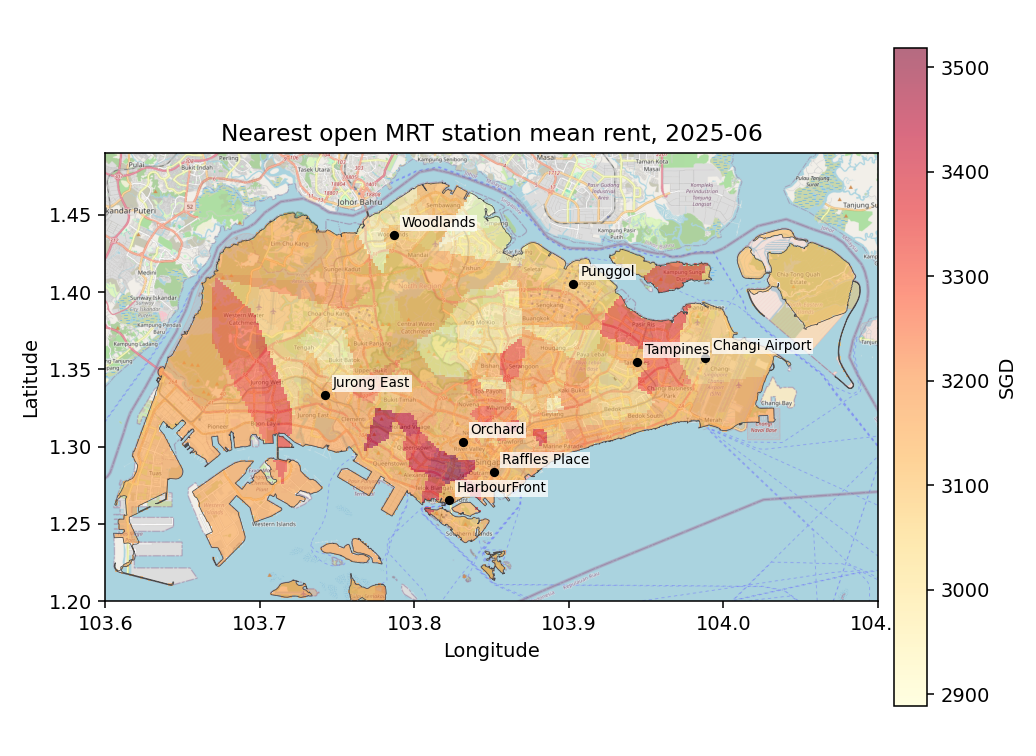
\includegraphics[width=0.92\linewidth,height=0.62\textheight,keepaspectratio]{map_mrt_2025-06.png}
\caption{Nearest open MRT station, June 2025.
Colour is the smoothed mean of labelled rents in the previous three months for that station.
Each area is one station.
The labelled table ends in March 2025, so the colours use March 2025 rents only.}
\label{fig:mrt-map}
\end{figure}

\subsection{Limits of the columns}
\label{sec:collimits}

\begin{itemize}
\item The maximum floor is the top floor of the block, not the flat's own floor.
Values of \(-1\) on floor and completion year are sentinels and are stored as null: 159 labelled rows, and none in the private test set.
\item The MRT file has no opening date.
A station marked open may have opened after January 2021.
In the trunk-prefix columns, planned stations and future-line prefixes stay out of the open-station distance.
\item About 20 MRT longitudes have only one to three decimal places.
Switching from the great-circle formula to a projected coordinate system does not repair that.
\item Great-circle distance is not walking time.
School and mall tables have no opening dates, and the school table has no university.
\item COE and stock columns are constant within an approval month.
January 2021 COE lags are null because December 2020 is missing.
The property basket is missing on early labelled rows because one constituent starts later.
\item Group means are target encodings of the previous three months of labelled rents.
They are not properties of a mall, a station, or a school.
January 2021 is null.
A mall mean covers rentals for which that mall is the nearest mall, not every flat inside a radius.
\item Empty postal codes, 285 blocks, have no postal-sector group and fall back to that quarter's island-wide mean once the three-month window contains any labelled rent.
\end{itemize}

\FloatBarrier
\section{Models}
\label{sec:models}

Four model approaches were fit.
Model~1 is a core CatBoost on the cleaned rental fields, with nested means, a random hold-out of the same size, and rolling one-year folds.
Model~2 is the rebuilt auxiliary CatBoost, under development folds and a 17-month assessment, with ridge checks beside it.
Model~3 is the multistage stack.
Model~4 is a global CatBoost with a property-adjusted rental
time index, developed in a separate fixed-split optimization series.
The best private-test result is add\_mrt.
Each model is stated as a motivation, a structure, and a performance.
Section~\ref{sec:headline} compares themafter those four accounts.
Table~\ref{tab:windows} names the windows before any score is quoted.
A score belongs to the window in its row.

\begin{table}[htbp]
\centering
\caption{Time windows.
The first four rows are the only names used for the multistage model.
Later rows are separate experiments.}
\label{tab:windows}
\small
\setlength{\tabcolsep}{3pt}
\begin{tabularx}{\textwidth}{@{}>{\raggedright\arraybackslash}p{0.30\textwidth}X@{}}
\toprule
Name & Definition \\
\midrule
Training set &
Labelled months through September 2024.
The only months that fit multistage parameters. \\
Validation set &
October--December 2024.
The only months that stop or choose the multistage model. \\
Test set &
January--March 2025.
Scored after that choice. \\
Private test set &
Unlabelled competition file after the labelled period.
A private-test RMSE did not stop or choose the multistage model. \\
Six-month hold-out &
Fit January 2021--September 2024 (132{,}802 rows).
Score October 2024--March 2025 (17{,}198 rows).
Core baselines. \\
One-year hold-out &
Fit January 2021--March 2024 (114{,}842 rows).
Score April 2024--March 2025 (35{,}158 rows). \\
Rolling folds &
Three expanding fits.
Each scores the next April--March year.
Table~\ref{tab:rolling}. \\
Development folds &
Fit through April 2022, October 2022, and April 2023.
Score the next six months: May--October 2022, November 2022--April 2023, and May--October 2023.
The development pooled RMSE combines squared error and row count across the three folds. \\
17-month assessment &
Fit through October 2023.
Score November 2023--March 2025. \\
\bottomrule
\end{tabularx}
\end{table}

The six-month hold-out fits on the same months as the training set.
Its 17{,}198 scored rows are the validation set and the test set placed end to end.
The one-year hold-out and the 17-month assessment cut the timeline in other places.
Development folds end in October 2023, so their scored months lie inside the months of the training set, and they are not the validation set.

\subsection{Model 1: Core CatBoost}
\label{sec:core-model}

\subsubsection{Motivation}

The competition file is mostly a later period than the labelled table.
March 2025 is the only overlapping calendar month.
A model that is judged on a random mix of years can look accurate while missing the shift it will face on a later month.
Model~1 therefore fits on earlier approval months and scores later ones.
A boosted tree is a reasonable next step after the nested means: flat type, town, time, and area interact, and the tree can split on a street or a flat model without a hand-built interaction list.

\subsubsection{Structure}

The comparison uses the six-month hold-out.
Four predictors are nested.
The global mean predicts the mean rent of the fitting portion for every scored row.
The town mean replaces that with the fitting-portion mean of the same town.
The town and flat-type mean uses the fitting-portion mean of that pair, and it falls back to the town mean and then the global mean when the pair is unseen.
All of those means use the fitting portion only.
The fourth predictor is a CatBoost regressor on the original property attributes and the derived time and age fields.
Categories are passed to the tree directly.
The tree uses 600 iterations, learning rate 0.05, depth 8, and random seed 42.
The time fields are approval year, calendar month, and the month index in Equation~\eqref{eq:month-index}.
Sine and cosine of the calendar month were added on the three rolling folds, so that December and January become neighbours in that pair of features.
The pair did not lower the rolling-fold RMSE on any fold, and the features were not kept.
Calendar month itself stays through the numerical month.
The fold-level cyclical numbers are in Appendix~\ref{app:cyclic}.

\subsubsection{Performance}

Table~\ref{tab:baseline-results} is the six-month hold-out.
On that six-month hold-out, town alone moves RMSE only from 795.76 to 778.62, town and flat type together move it to 565.58, and CatBoost reaches 454.29.
Relative to the global mean, that is a reduction of about 42.9\% in six-month hold-out RMSE.
The interaction of property type, location, time, and the other dwelling fields carries information that the historical averages do not.

\begin{table}[htbp]
\centering
\caption{Core baselines on the six-month hold-out, October 2024--March 2025, after a fit through September 2024.
Six-month hold-out RMSE is in SGD of monthly rent.}
\label{tab:baseline-results}
\small
\begin{tabular}{lr}
\toprule
Model & RMSE \\
\midrule
Global mean & 795.76 \\
Town mean & 778.62 \\
Town + flat type mean & 565.58 \\
CatBoost & 454.29 \\
\bottomrule
\end{tabular}
\end{table}

The same CatBoost configuration was also scored on a random hold-out with the same number of fitting rows and the same number of scored rows.
Table~\ref{tab:random-temporal} compares the two schemes.
The random hold-out has RMSE 476.25, about 22~SGD higher than the six-month hold-out RMSE of 454.29.
The chronological split was kept because its information flow matches a later scoring period, not because it produces a lower number.
The mean errors differ in a more specific way.
Mean error is predicted rent minus observed rent.
The random hold-out has mean error \(-6.64\).
The six-month hold-out has mean error \(-36.29\): the model underpredicts later rents by about 36~SGD on average.
Mixing all years hides part of that bias.

\begin{table}[htbp]
\centering
\caption{Core CatBoost on a chronological six-month hold-out and on a random hold-out of the same size.
RMSE is the six-month hold-out RMSE or the random-hold-out RMSE, in SGD of monthly rent.
Mean error is predicted minus observed rent, in SGD.}
\label{tab:random-temporal}
\small
\begin{tabular}{lrr}
\toprule
Scheme & RMSE & Mean error \\
\midrule
Six-month hold-out & 454.29 & $-36.29$ \\
Random hold-out & 476.25 & $-6.64$ \\
\bottomrule
\end{tabular}
\end{table}

\paragraph{Rolling one-year folds.}
\label{sec:rolling}

One hold-out can be an accident of the months it covers.
Three expanding folds each score a full April--March year, so every calendar month appears once in the scored year.
Table~\ref{tab:rolling} is the result for the same core CatBoost.
Rolling-fold RMSE falls from 719.52 to 599.59 to 477.47.
The mean errors are \(-370.41\), \(-146.57\), and \(-35.74\).
The earliest fit underpredicts the next year by a large margin.
The latest fold is much closer to zero mean error.
The rental level moved across years, and one pooled cross-validation number would hide that movement.
The most recent one-year fold is the primary long window for Model~1.
The earlier folds are the robustness check.
Fold 3 scores April 2024 through March 2025 after a fit through March 2024.
That scored year mixes months which, under the multistage names, sit in the training set, the validation set, and the test set.
The one-year hold-out RMSE of 477.47 belongs to Model~1.
It is not a validation RMSE and it is not a test RMSE.

\begin{table}[htbp]
\centering
\caption{Expanding-window core CatBoost on the rolling folds.
Each scored period is one April--March year.
Rolling-fold RMSE is in SGD of monthly rent.}
\label{tab:rolling}
\small
\setlength{\tabcolsep}{4pt}
\begin{tabular}{@{}llrrrr@{}}
\toprule
Fold & Fit & Scored & Fit rows & Scored rows & RMSE \\
\midrule
1 & Jan 2021--Mar 2022 & Apr 2022--Mar 2023 & 46{,}756 & 32{,}204 & 719.52 \\
2 & Jan 2021--Mar 2023 & Apr 2023--Mar 2024 & 78{,}960 & 35{,}882 & 599.59 \\
3 & Jan 2021--Mar 2024 & Apr 2024--Mar 2025 & 114{,}842 & 35{,}158 & 477.47 \\
\bottomrule
\end{tabular}
\end{table}

The year-to-year change in Table~\ref{tab:rolling} is much larger than the change from the cyclical pair, which is why that pair was dropped in Section~\ref{sec:core-model}.

\paragraph{Where the model errs.}

On the six-month hold-out, monthly CatBoost RMSE stays between 438.22 and 471.08 (Table~\ref{tab:monthly-errors}).
Mean error is negative in every month, and the underprediction is larger again in February and March 2025.
That pattern agrees with the rolling folds: forward prediction is sensitive to the level of the market.
The monthly table does not by itself identify why the level moved.

\begin{table}[htbp]
\centering
\caption{Monthly core CatBoost errors on the six-month hold-out.
Six-month hold-out RMSE and MAE are in SGD of monthly rent.
Mean error is predicted minus observed rent, in SGD.}
\label{tab:monthly-errors}
\small
\begin{tabular}{lrrr}
\toprule
Month & RMSE & MAE & Mean error \\
\midrule
Oct 2024 & 438.22 & 326.54 & $-35.05$ \\
Nov 2024 & 464.91 & 330.08 & $-22.80$ \\
Dec 2024 & 447.66 & 325.29 & $-18.14$ \\
Jan 2025 & 471.08 & 346.60 & $-37.51$ \\
Feb 2025 & 453.18 & 338.46 & $-48.63$ \\
Mar 2025 & 449.69 & 332.37 & $-53.33$ \\
\bottomrule
\end{tabular}
\end{table}

Errors also differ by flat type (Table~\ref{tab:flat-type-errors}).
Among types with a substantial count, executive flats have the highest six-month hold-out RMSE, then 5-room flats.
The 1-room row has seven scored leases and is not interpreted.
The executive gap is one reason to look at building and location information beyond flat type.

\begin{table}[htbp]
\centering
\caption{Core CatBoost errors by flat type on the six-month hold-out.
RMSE is the six-month hold-out RMSE, in SGD of monthly rent.}
\label{tab:flat-type-errors}
\small
\begin{tabular}{lrrr}
\toprule
Flat type & Scored rows & RMSE & MAE \\
\midrule
Executive & 852 & 537.59 & 394.18 \\
5-room & 3{,}908 & 471.58 & 334.12 \\
4-room & 6{,}268 & 456.66 & 335.12 \\
2-room & 476 & 434.03 & 312.54 \\
3-room & 5{,}687 & 426.74 & 323.41 \\
1-room & 7 & 461.55 & 428.94 \\
\bottomrule
\end{tabular}
\end{table}

Table~\ref{tab:baseline-importance} is a diagnostic of this fitted baseline, not a causal ranking.
Flat type, the month index, and town account for most of the reported importance.
The month index agrees with the temporal-shift results: time is part of the hold-out design, not only another covariate.
Several columns encode related facts, so the shares are not independent effects.
The importance names are the names recorded for this preliminary model.
Furnished status and the fee received zero importance here, which agrees with the audit that both are constant.

\begin{table}[htbp]
\centering
\caption{Leading feature importances in the preliminary core CatBoost.}
\label{tab:baseline-importance}
\small
\begin{tabular}{lr}
\toprule
Feature & Importance \\
\midrule
\texttt{FLAT\_TYPE} & 28.04 \\
\texttt{MONTH\_INDEX} & 22.62 \\
\texttt{TOWN} & 16.69 \\
\texttt{FLOOR\_AREA\_SQM} & 7.62 \\
\texttt{STREET} & 5.27 \\
\texttt{LEASE\_COMMENCE\_DATE} & 4.71 \\
\texttt{FLAT\_MODEL} & 4.71 \\
\texttt{FLAT\_AGE} & 3.13 \\
\texttt{BLOCK} & 2.92 \\
\texttt{RENT\_YEAR} & 2.32 \\
\texttt{RENT\_MONTH} & 1.99 \\
\bottomrule
\end{tabular}
\end{table}

\subsection{Model 2: Auxiliary CatBoost}
\label{sec:aux-model}

\subsubsection{Motivation}

Model~2 asks whether the auxiliary families lower the development pooled RMSE or the 17-month RMSE once dwelling, address, and calendar fields are already present.
It keeps the same tree family as Model~1 and changes the column set.

\subsubsection{Structure}

All tree configurations share one recorded hyperparameter setting.
Mean and ridge checks use the same windows.
A positive addition is the original-address RMSE minus the augmented RMSE on the same window.
A positive removal cost is the ablated RMSE minus the full-model RMSE on that same window.
Those windows are the development pooled RMSE and the 17-month RMSE.
The development pooled RMSE combines squared error and row count across the three development folds.
It is not the average of three development-fold RMSE values.

Two macro timings are reported.
Cutoff-frozen holds the scored months' macro descriptors at the feature vector available at the preceding cutoff.
Provided-lagged conditions each rental month on supplied observations from the preceding completed month.
Provided-lagged is a batch setting in which that lag is available.
Missing source observations are left missing.
Stock principal components are learned with one row per fitting month, not with the rental row repeated once per flat.

Before the configuration table, each numeric spatial exposure was screened on its own, on development data through October 2023, after controls for area, log area, lease age, flat type, flat model, town, and approval-month fixed effects.
The exposures are not entered jointly.
Intervals are clustered by address.
The coefficients in Table~\ref{tab:assoc} are SGD per original feature unit.
They are conditional associations.
They are not causal premiums for a facility: unit floor, renovation, household composition, and other neighbourhood differences can remain.
Building age's interval includes zero.
Distance to the central business district, to an open MRT station, and to a mall have negative intervals.
The two secondary-school definitions do not share a sign.
Figure~\ref{fig:bands} shows zero-centred adjusted-rent residuals in quantile bins of distance, without adding back a baseline rent and without choosing a reference band.
The pointwise address-cluster intervals omit uncertainty from the control fit.

\begin{table}[htbp]
\centering
\caption{Conditional associations on development data through October 2023.
Each spatial column is entered separately.
Intervals cluster by address.
Units are SGD per original feature unit.}
\label{tab:assoc}
\small
\begin{tabular}{lrr}
\toprule
Spatial variable (unit) & SGD per unit & 95\% interval \\
\midrule
Maximum block floor (floor) & $+6.49$ & $[5.25,\ 7.73]$ \\
Building age (year) & $-1.36$ & $[-4.86,\ 2.13]$ \\
CBD distance (km) & $-31.22$ & $[-37.04,\ -25.40]$ \\
Open MRT distance (km) & $-132.52$ & $[-147.89,\ -117.16]$ \\
Mall distance (km) & $-97.26$ & $[-109.04,\ -85.49]$ \\
Primary distance (km) & $-22.50$ & $[-42.27,\ -2.74]$ \\
Secondary S1--S4 (km) & $-36.82$ & $[-43.30,\ -30.35]$ \\
Secondary S1--S5 (km) & $+19.22$ & $[4.72,\ 33.71]$ \\
\bottomrule
\end{tabular}
\end{table}

\begin{figure}[htbp]
\centering
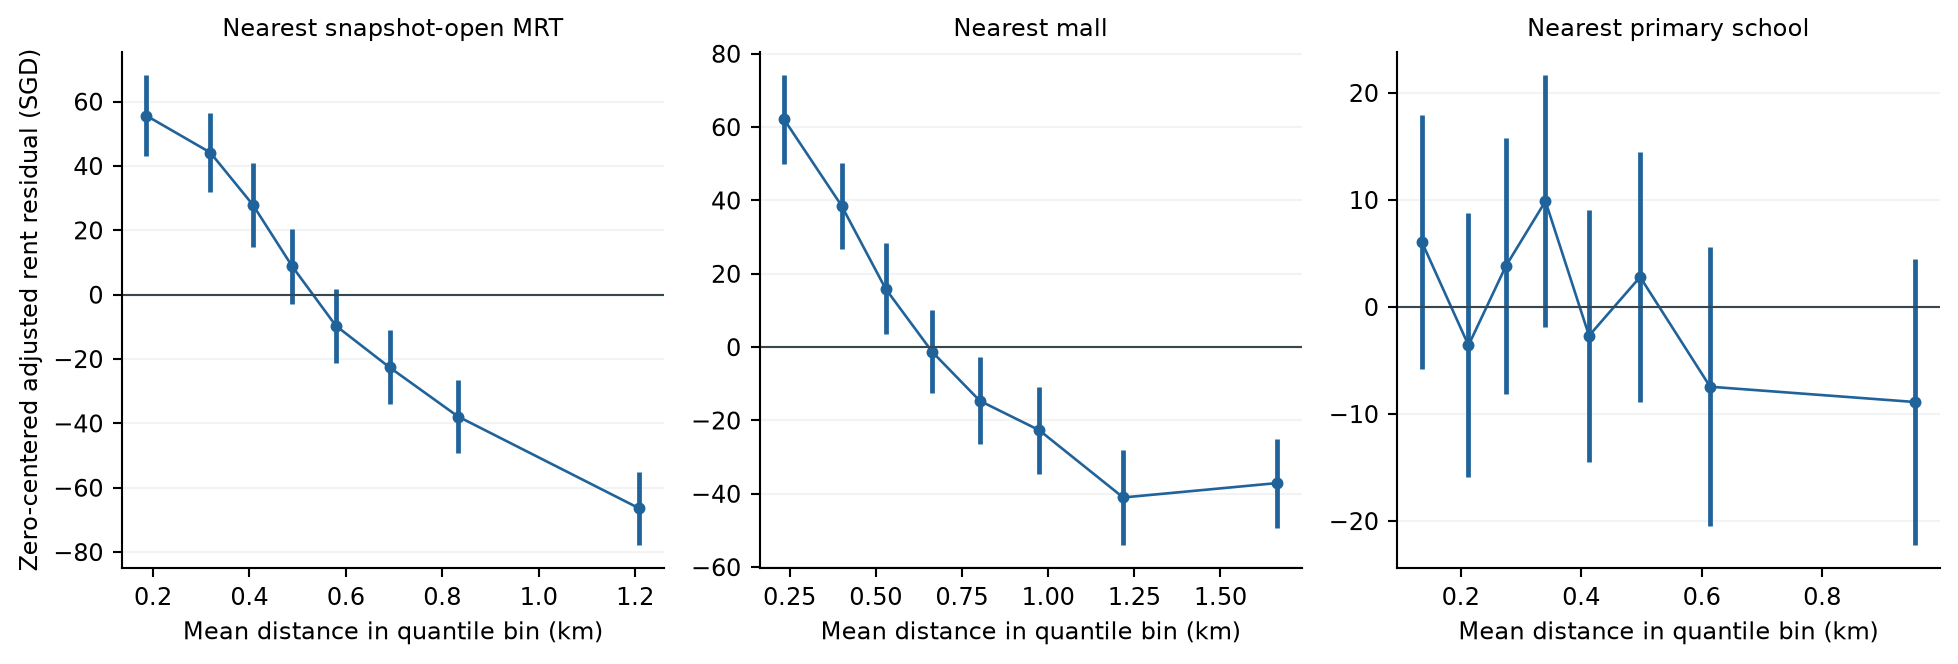
\includegraphics[width=0.98\linewidth,height=0.55\textheight,keepaspectratio]{rebuilt_conditional_distance_bands.png}
\caption{Zero-centred adjusted-rent residuals by distance bin, on the development screen.
The curves do not add back baseline rent.}
\label{fig:bands}
\end{figure}

\subsubsection{Performance}

Tables~\ref{tab:cutoff} and~\ref{tab:lagged} are the locked CatBoost configurations.
Among the predefined main CatBoost configurations, excluding the retrospective adjusted-price sensitivity, the lowest development pooled RMSE belongs to add-MRT.
That ranking uses the development results only.
On the 17-month assessment, add-MRT has 17-month RMSE 499.53 and original plus address has 17-month RMSE 501.83.
All-auxiliary has a higher 17-month RMSE in both macro timings: 517.51 cutoff-frozen and 553.50 provided-lagged.
The add-MRT row does not depend on the macro timing, and it is the same number in both tables.
Ridge all-auxiliary has a lower development pooled RMSE than add-MRT.
The development ranking quoted above is the CatBoost ranking, not a ranking across model families.
The 17-month assessment fits through October 2023.
That 17-month RMSE is not comparable with the six-month hold-out RMSE of 454.29, which fits through September 2024.

\begin{table}[htbp]
\centering
\caption{Cutoff-frozen macro.
The development pooled RMSE combines squared error and row count across the three development folds.
The 17-month assessment fits through October 2023 and scores November 2023--March 2025.
The 17-month RMSE is not the six-month hold-out.
Adjusted-price sensitivity is retrospective and is excluded from the CatBoost ranking.}
\label{tab:cutoff}
\small
\begin{tabular}{lrr}
\toprule
Configuration & Dev.\ pooled RMSE & 17-month RMSE \\
\midrule
Training mean & 939.64 & 894.19 \\
Ridge, original + address & 632.91 & 677.64 \\
Ridge, all auxiliary & 615.95 & 544.21 \\
Original dwelling & 640.49 & 509.53 \\
Original + address & 627.84 & 501.83 \\
All main auxiliary & 631.09 & 517.51 \\
Add MRT & 622.58 & 499.53 \\
Adjusted-price sensitivity & 640.58 & 520.05 \\
\bottomrule
\end{tabular}
\end{table}

\begin{table}[htbp]
\centering
\caption{Provided-lagged macro.
Windows match Table~\ref{tab:cutoff}.
Configurations that do not use the macro timing match that table.}
\label{tab:lagged}
\small
\begin{tabular}{lrr}
\toprule
Configuration & Dev.\ pooled RMSE & 17-month RMSE \\
\midrule
Training mean & 939.64 & 894.19 \\
Ridge, original + address & 632.91 & 677.64 \\
Ridge, all auxiliary & 613.40 & 509.29 \\
Original dwelling & 640.49 & 509.53 \\
Original + address & 627.84 & 501.83 \\
All main auxiliary & 643.79 & 553.50 \\
Add MRT & 622.58 & 499.53 \\
Adjusted-price sensitivity & 661.29 & 549.25 \\
\bottomrule
\end{tabular}
\end{table}

Figure~\ref{fig:families} draws the addition and the removal of families under both macro timings.
Figure~\ref{fig:assess} is the monthly error on the 17-month assessment.
Figure~\ref{fig:shap} shows leading attributions of the fitted full model on the recorded assessment sample.
They locate predictive signal in dwelling attributes, calendar, and location.
They are attributions of that fit, not a causal decomposition.

\begin{figure}[htbp]
\centering
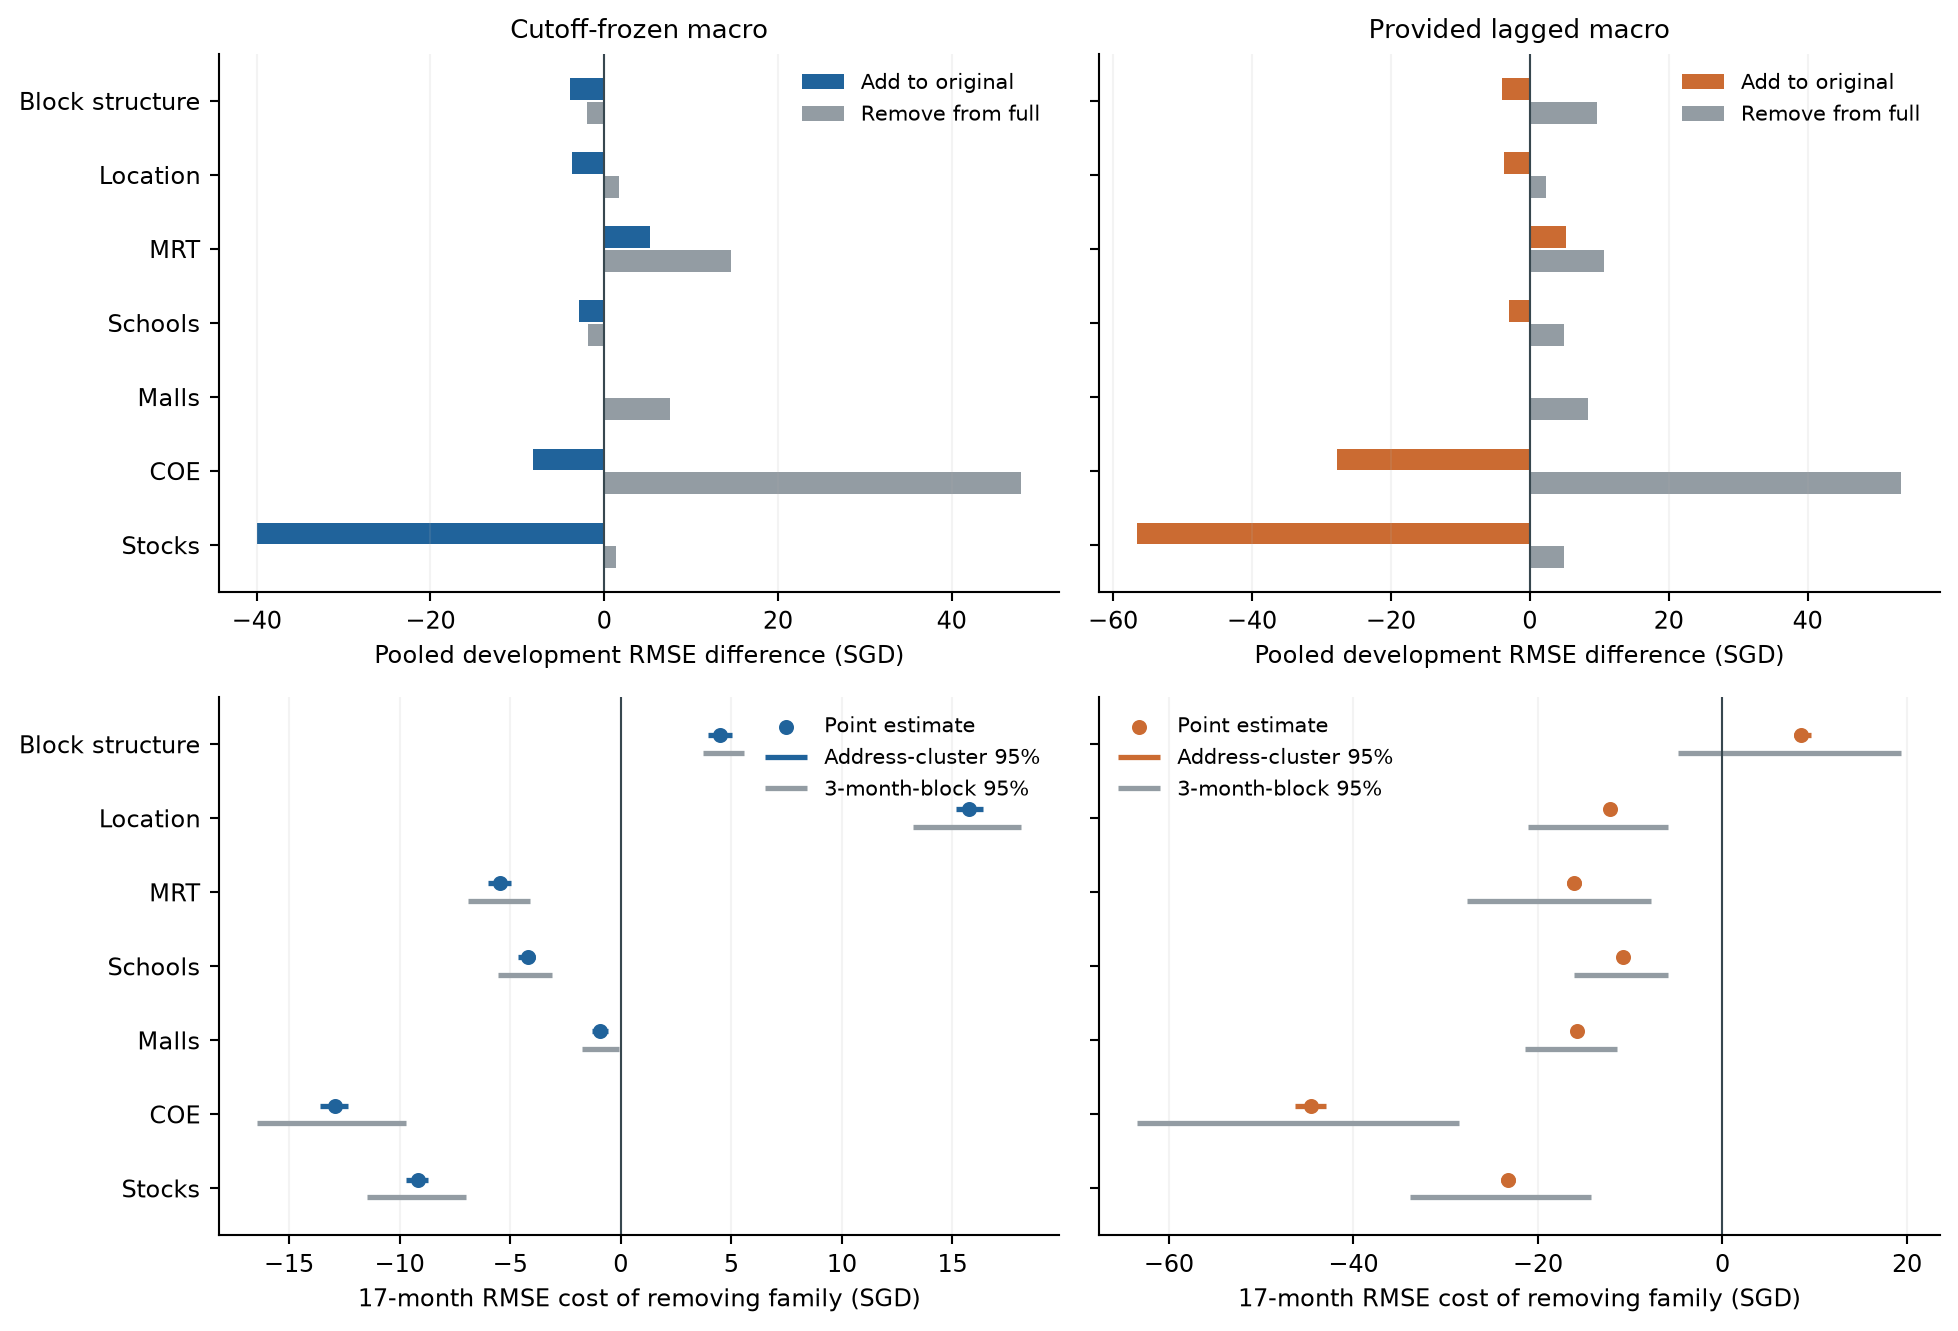
\includegraphics[width=0.98\linewidth,height=0.52\textheight,keepaspectratio]{rebuilt_family_contributions.png}
\caption{Family additions and removals.
A positive addition is the original-address RMSE minus the augmented RMSE on the same window.
A positive removal cost is the ablated RMSE minus the full-model RMSE on that same window.
The development pooled RMSE combines squared error and row count.
The lower panels are the 17-month assessment.}
\label{fig:families}
\end{figure}

\begin{figure}[htbp]
\centering
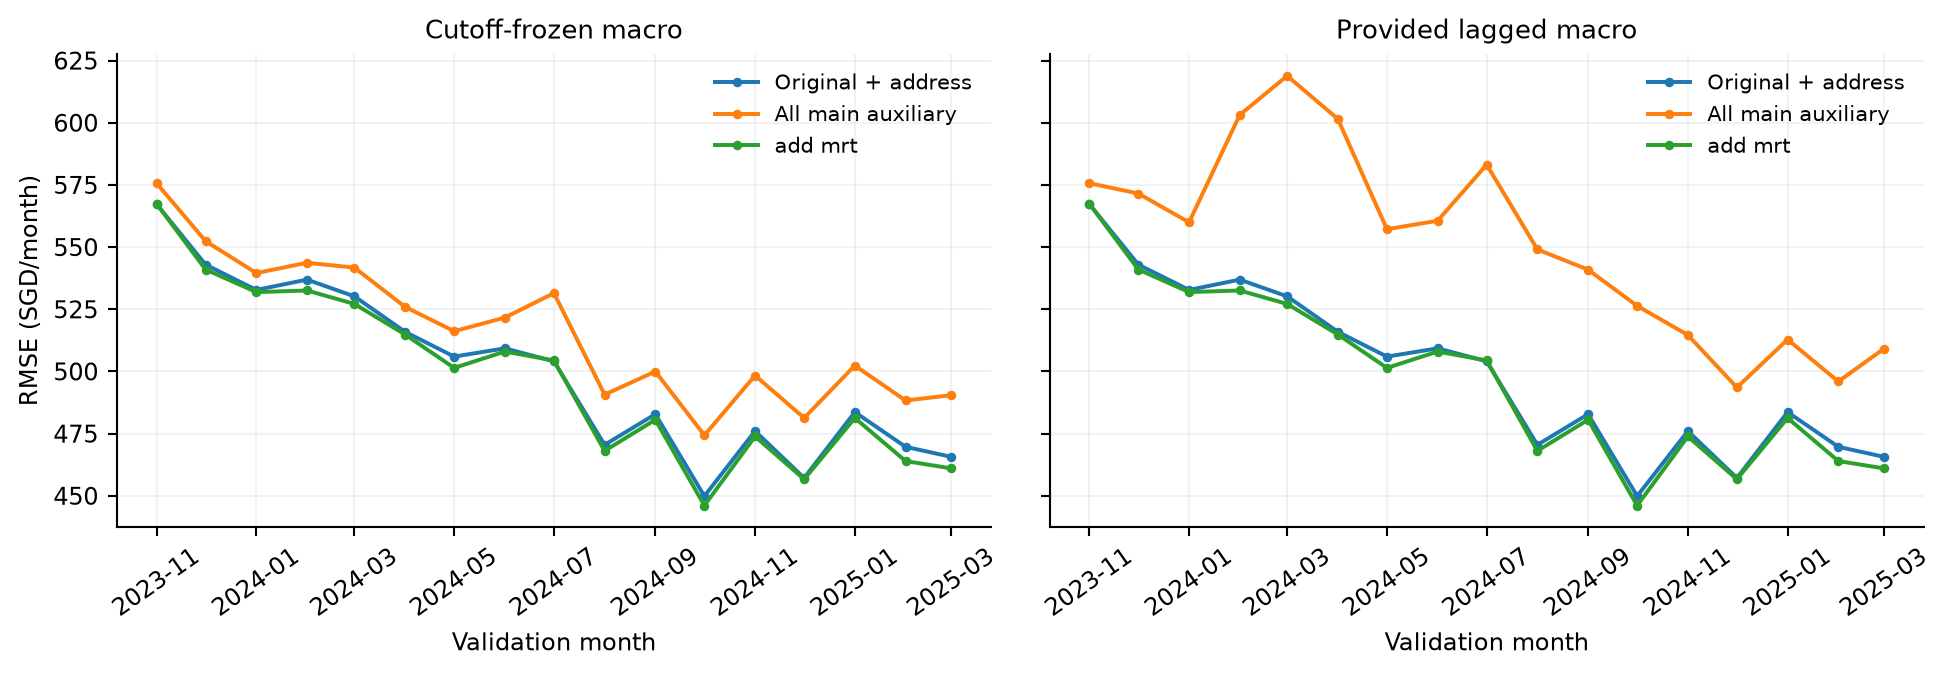
\includegraphics[width=0.98\linewidth,height=0.52\textheight,keepaspectratio]{rebuilt_17month_errors.png}
\caption{Monthly error on the 17-month assessment, November 2023--March 2025, after a fit through October 2023.}
\label{fig:assess}
\end{figure}

\begin{figure}[htbp]
\centering
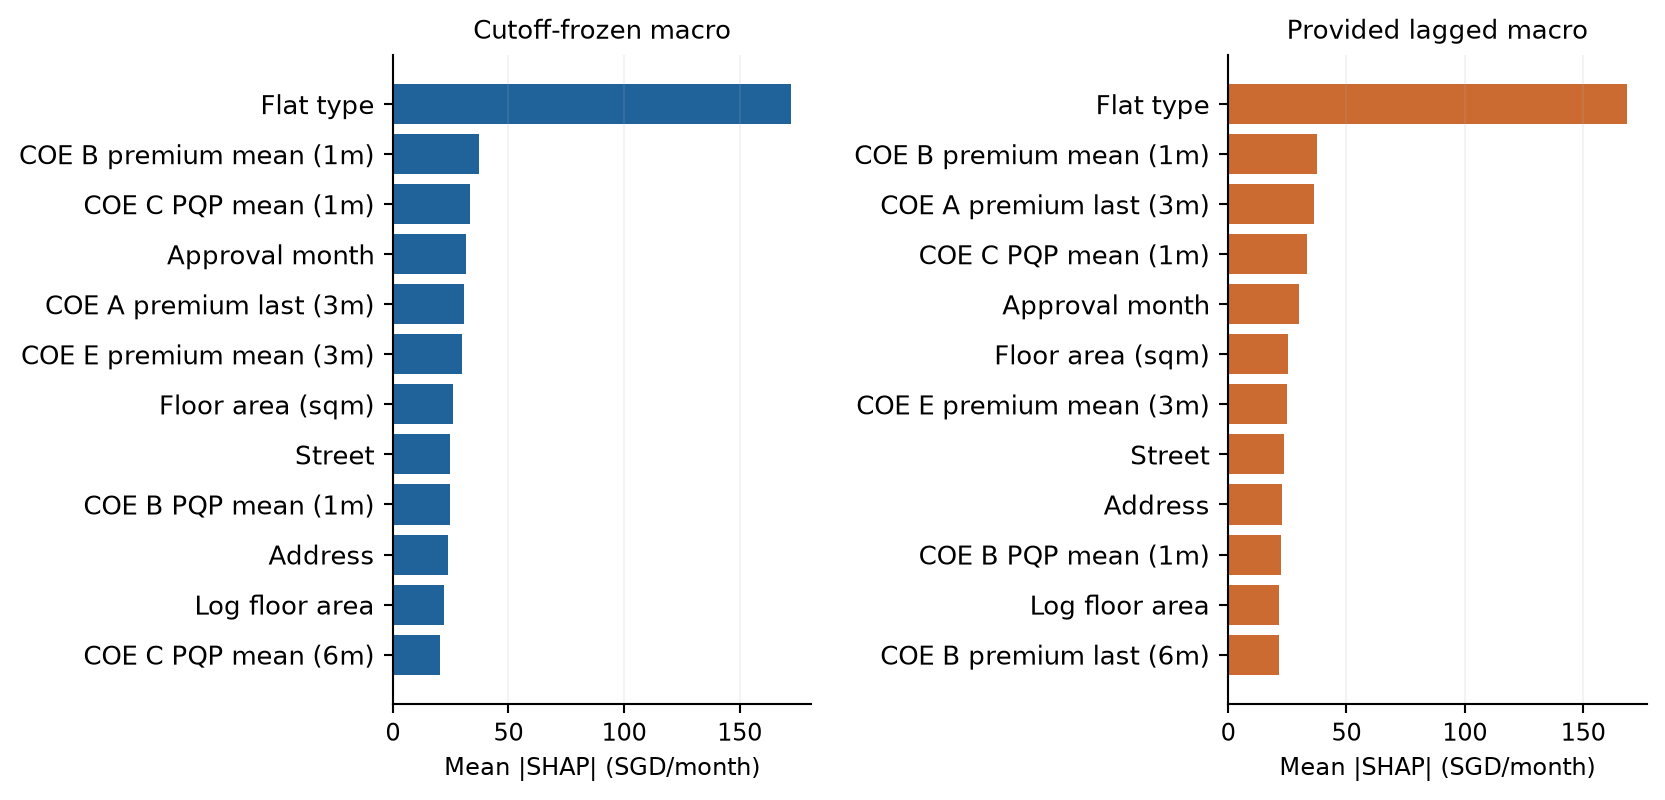
\includegraphics[width=0.98\linewidth,height=0.52\textheight,keepaspectratio]{rebuilt_model_attributions.png}
\caption{Leading full-model attributions on the recorded assessment sample.}
\label{fig:shap}
\end{figure}

\subsection{Model 3: Multistage model}
\label{sec:stack}

\subsubsection{Motivation}

Model~3 is the multistage stack.
It separates a town-month path from the within-town gap, and then converts both into monthly rent.
The motivation is the Model~1 result that town, flat type, and the month index already carry most of the baseline importance, while a single town mean is still a weak predictor of the flat.
Flats in one town move together through the month, and a flat's own site and type explain the rest.
A recurrent network is a reasonable model of the shared path because the path is an ordered series and the hidden state can carry the economic inputs already observed before the month being predicted.
A tree is a reasonable model of one gap because the within-town columns include names and codes.
A Gaussian mixture is a reasonable model of the other gap because the remaining difference still varies smoothly inside the town.
The two gap models are fit separately and do not see each other, so the shared network receives two estimates of the same residual rather than one estimate passed through the other.
One shared network, not one network per town, maps those pieces to monthly rent.

\paragraph{Why the region is a town.}
A partition check compared five geographic units as the cell of a month mean, on the training set.
A cell is one geographic unit in one approval month.
Table~\ref{tab:cells} is that count.
Town has no missing rows.
A typical town-month cell has about 110 flats, and 5.9\% of town-month cells have fewer than 30.
Planning areas are thinner.
Postal districts and postal sectors also drop 4{,}685 rows with no postal code.
Postal sectors then have a median of 34 rows, and 43.5\% of their cells are under 30.
Town is fine enough that towns differ, and it is still large enough that a typical cell is not a handful of leases.

\begin{table}[htbp]
\centering
\caption{Cells in the training set.
A cell is one geographic unit in one approval month.
``Under 30'' is the share of cells with fewer than 30 flats.}
\label{tab:cells}
\small
\setlength{\tabcolsep}{4pt}
\begin{tabular}{lrrrrr}
\toprule
Unit & Groups & Missing rows & Cells & Median rows & Under 30 \\
\midrule
Region & 5 & 0 & 225 & 638 & 0\% \\
Town & 26 & 0 & 1{,}170 & 110.5 & 5.9\% \\
Planning area & 31 & 0 & 1{,}341 & 96 & 19.2\% \\
Postal district & 24 & 4{,}685 & 1{,}035 & 78 & 25.7\% \\
Postal sector & 53 & 4{,}685 & 2{,}261 & 34 & 43.5\% \\
\bottomrule
\end{tabular}
\end{table}

Figure~\ref{fig:town-may} is the observed town mean of rent per square metre in May 2024.
The colour is that observed mean, not a forecast, and the map was not scored.
Central and southern towns are darker than the north and west, so the town mean is not one island-wide number.

\begin{figure}[htbp]
\centering
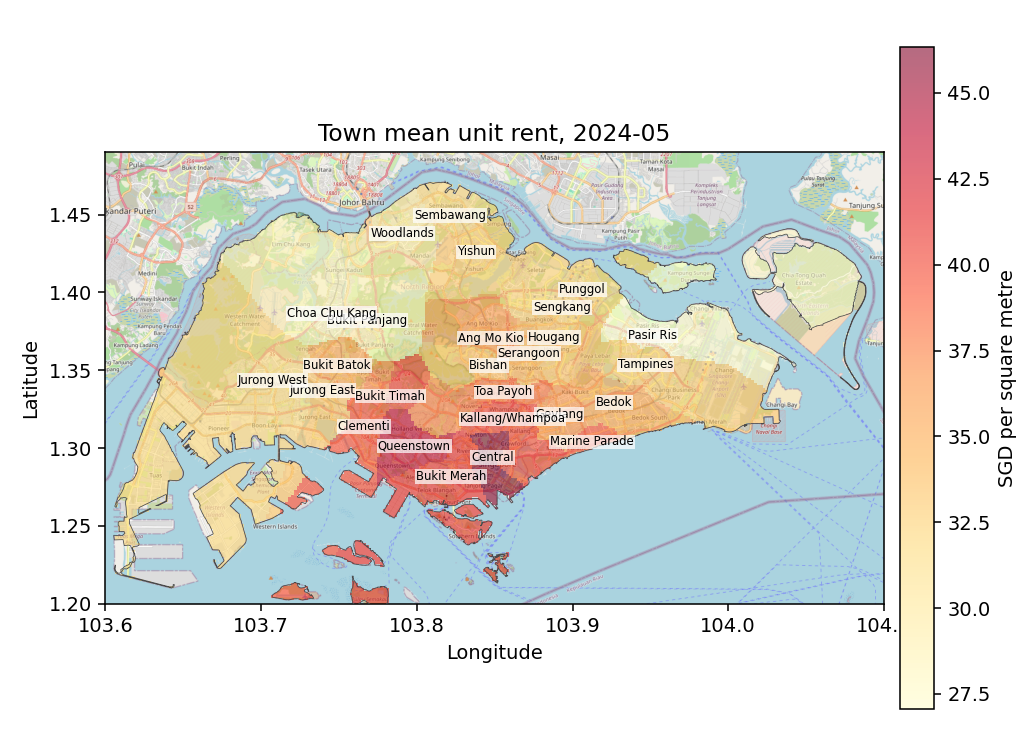
\includegraphics[width=0.92\linewidth,height=0.58\textheight,keepaspectratio]{town_unit_mean_2024-05.png}
\caption{May 2024 mean of rent per square metre by town.
Each patch is the town of the nearest HDB block.
The colour is the unweighted mean of the flats approved in that month.
The map was not scored.}
\label{fig:town-may}
\end{figure}

Table~\ref{tab:partition} is a ridge of the town-month mean of monthly rent, in SGD, weighted by the cell.
Town indicators plus a month index leave a large dollar cell RMSE on both the validation set and the test set.
Adding the category-C COE premium and the bank-basket level removes most of that dollar cell RMSE.
Adding the property-basket level lowers the validation cell RMSE further, from 94.37 to 93.36, and lowers the test cell RMSE from 112.85 to 103.31.
Using all 15 COE and stock columns, including changes, bid ratios, and returns, raises the validation cell RMSE to 104.81 and the test cell RMSE to 229.70.
Month-to-month COE changes and bid ratios alone do not beat the month index on the validation cell RMSE or the test cell RMSE.
A separate month slope for each town was worse than one shared slope.
The economy inputs adopted for the region mean are therefore the month index and those three level series.
These figures are dollar cell RMSEs of the town-month mean of monthly rent.
They are not the per-square-metre cell RMSEs of the recurrent network reported below.

\begin{table}[htbp]
\centering
\caption{Weighted cell RMSE of the town-month mean of monthly rent, in SGD.
The validation set is October--December 2024.
The test set is January--March 2025 and did not choose the specification.
These are dollar cell RMSEs, not per-square-metre cell RMSEs.}
\label{tab:partition}
\small
\begin{tabular}{lrr}
\toprule
Specification & Validation & Test \\
\midrule
Town and month index & 291.65 & 366.09 \\
Plus COE C premium and bank basket & 94.37 & 112.85 \\
Plus property basket & 93.36 & 103.31 \\
All 15 COE and stock columns & 104.81 & 229.70 \\
\bottomrule
\end{tabular}
\end{table}

\subsubsection{Structure}

Figure~\ref{fig:stack} is the architecture.

\begin{figure}[htbp]
\centering
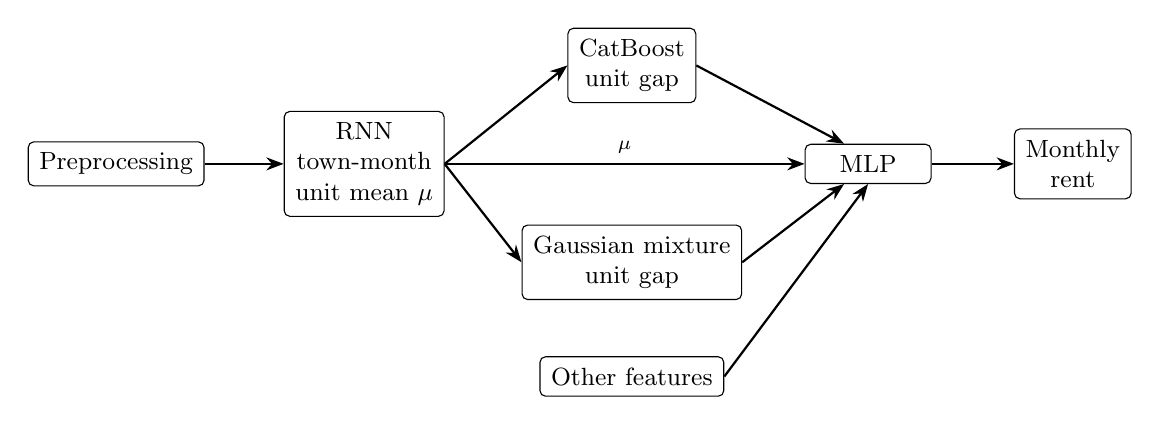
\begin{tikzpicture}[
  font=\small,
  box/.style={draw, rounded corners=2pt, align=center, inner sep=4pt},
  arr/.style={-{Stealth[length=2.2mm]}, thick}
]
\node[box] (prep) at (0,0) {Preprocessing};
\node[box] (rnn) at (3.15,0) {RNN\\town-month\\unit mean $\mu$};
\node[box] (cb) at (6.55,1.25) {CatBoost\\unit gap};
\node[box] (gmm) at (6.55,-1.25) {Gaussian mixture\\unit gap};
\node[box] (feat) at (6.55,-2.7) {Other features};
\node[box, minimum width=16mm] (mlp) at (9.55,0) {MLP};
\node[box] (out) at (12.15,0) {Monthly\\rent};
\draw[arr] (prep) -- (rnn);
\draw[arr] (rnn.east) -- (cb.west);
\draw[arr] (rnn.east) -- (gmm.west);
\draw[arr] (cb.east) -- (mlp.140);
\draw[arr] (gmm.east) -- (mlp.220);
\draw[arr] (rnn.east) -- node[above, font=\scriptsize] {$\mu$} (mlp.west);
\draw[arr] (feat.east) -- (mlp.south);
\draw[arr] (mlp) -- (out);
\end{tikzpicture}
\caption{Multistage prediction.
The recurrent network estimates the town-month rent per square metre.
CatBoost and the Gaussian mixture are fit separately and estimate the unit-price gap from that mean.
One shared multilayer perceptron receives the mean, both gaps, floor area, and the flat's other features, and it outputs monthly rent.}
\label{fig:stack}
\end{figure}

\paragraph{Region mean.}
The region model predicts the town-month mean of rent per square metre, monthly rent divided by floor area, with equal weight per flat.
Each town has its own network.
The network is a recurrent net with hidden size 16, three layers, and a tanh nonlinearity, followed by a linear map from 16 units to one output.
The input is the time index and the economic trend already observed before the month being predicted.
The network does not see the true subsequent town-month rents.
The hidden state carries the earlier economic inputs.
Running the sequence from 2021 is required: a zero initial state would drop that history.
The training schedule is in Appendix~\ref{app:dollar}.

\paragraph{Within-town gap.}
CatBoost and a Gaussian mixture are fit separately, one pair per town, to the same target: unit rent minus the recurrent-network town-month unit mean.
Neither model sees the other's output.
The mixture is a full-covariance Gaussian mixture in five dimensions: latitude and longitude standardized inside the town, flat-type rank and flat-model rank standardized inside the town, and the per-square-metre residual.
The residual is a coordinate.
It may be negative, so a component can sit below the region mean.
The prediction is the responsibility-weighted conditional mean of that residual given the location and the two ranks.
It is not a probability multiplied by the region mean.
The component-count rule, the tree's column list, and the earlier dollar location check are in Appendix~\ref{app:gap}.
Both gap predictions are turned back into a monthly rent by adding the gap to the recurrent-network mean and multiplying by floor area.
Both gaps are then passed to the shared network.

Figure~\ref{fig:bukit} is Bukit Panjang, drawn from the saved stack mixture.
The town kept six components.
The surface is the mixture's conditional per-square-metre gap at that town's mean flat-type rank and mean flat-model rank.
It is the predicted gap from the region mean, not the rent itself.
December 2024 points are that month's unit rent minus Bukit Panjang's true December unit mean.
The true December mean is 30.19~SGD per square metre, and the recurrent-network region mean is 30.71.
A point and the cell under it do not use the same baseline.
The point uses the true December mean.
The surface uses the predicted gap from the region mean.
The colour scale is shared across towns, symmetric about zero, at the 98th percentile of absolute values.
A cell more than 400\,m from a flat in the training set is blank.
The figure was not scored.

\begin{figure}[htbp]
\centering
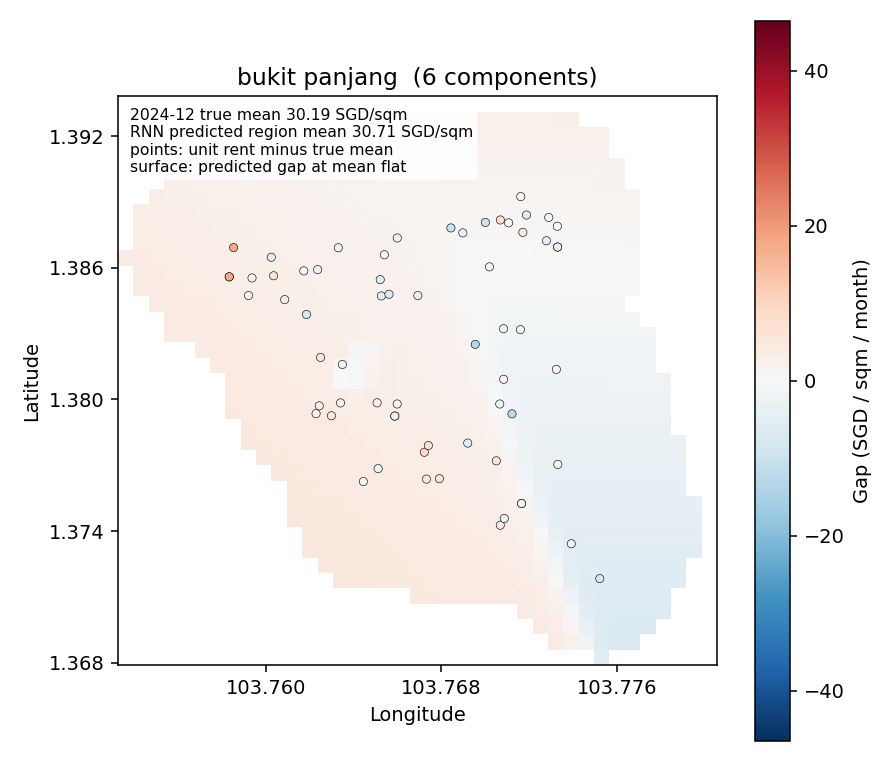
\includegraphics[width=0.86\linewidth,height=0.62\textheight,keepaspectratio]{bukit_panjang.png}
\caption{Bukit Panjang.
The surface is the conditional per-square-metre gap at the town's mean flat ranks.
December 2024 points are unit rent minus that town's true December unit mean, 30.19~SGD per square metre.
The recurrent-network region mean for that month is 30.71.
Cells farther than 400\,m from a flat in the training set are blank.
The figure was not scored.}
\label{fig:bukit}
\end{figure}

\paragraph{The shared network.}
One multilayer perceptron sees every town.
It is not trained separately by town.
The town-specific pieces it receives are the recurrent-network mean, the CatBoost gap, and the mixture gap, together with floor area and the flat's other features.
The network has a linear map to 128 units, a ReLU, dropout 0.1, a linear map to 64 units, a ReLU, dropout 0.1, and a linear map to one output.
The output is monthly rent.
Floor area is not applied again after the network.
The input list and the optimiser are in Appendix~\ref{app:gap}.
The six group-mean columns are not among those inputs.
A different 40-column CatBoost keeps five of them.
That model is not the town stage, and the stack does not replace it.

\subsubsection{Performance}

Weighted cell RMSE of the unit-price mean is 0.9707 on the validation set and 1.0897 on the test set.
The weights are the number of flats in the cell.
These validation and test figures are per-square-metre cell RMSEs of the town-month unit-price mean.
They are not the flat-level RMSE of monthly rent, and they are not comparable with a dollar cell RMSE.
The test-set per-square-metre cell RMSE did not choose the network.

Table~\ref{tab:gap} records the flat-level validation RMSE and test RMSE of the two gap models after the gap is added back to the recurrent-network mean and multiplied by floor area.
The per-square-metre columns and the rent columns are the same predictions expressed in two units.
They are not the validation or test per-square-metre cell RMSE of the region mean.
On the validation set, the town CatBoost has a lower validation rent RMSE than the mixture.
On the test set, it has a lower test rent RMSE than the mixture.
The test set did not choose either model.

\begin{table}[htbp]
\centering
\caption{Flat-level RMSE after adding the predicted gap to the recurrent-network unit mean.
The rent columns multiply that unit price by floor area.
The validation set is October--December 2024.
The test set is January--March 2025 and did not choose either model.}
\label{tab:gap}
\small
\setlength{\tabcolsep}{5pt}
\begin{tabular}{lrrrr}
\toprule
 & \multicolumn{2}{c}{SGD per square metre} & \multicolumn{2}{c}{Monthly rent, SGD} \\
\cmidrule(lr){2-3}\cmidrule(lr){4-5}
Model & Validation & Test & Validation & Test \\
\midrule
CatBoost & 5.3811 & 5.4562 & 455.06 & 469.19 \\
Mixture & 5.7707 & 5.8380 & 490.02 & 502.48 \\
\bottomrule
\end{tabular}
\end{table}

Training runs for at most 100 epochs.
After each epoch the validation RMSE of monthly rent is computed.
If that RMSE does not fall by more than \(10^{-6}\) for 10 consecutive epochs, training stops and the weights from the best validation epoch are restored.
The kept run stops at epoch 8.
Validation RMSE is 448.24.
Test RMSE is 462.87.
Training RMSE on the training set is 461.25.
The test set did not choose the epoch.
A private-test RMSE did not choose it either.
On the validation set, the validation RMSE 448.24 is lower than either gap model's validation rent RMSE in Table~\ref{tab:gap}.
On the test set, the test RMSE 462.87 is lower than either gap model's test rent RMSE in that table.
The CatBoost gap on the training set is the saved full model's prediction on its own training rows, because out-of-fold vectors were not stored.
Validation, test, and private-test CatBoost features are that same full model applied to those rows.

\FloatBarrier
\subsection{Model 4: Global CatBoost with a Rental Time Index}
\label{sec:time-index-model}

\subsubsection{Motivation}

Model~4 asks whether a shared model of monthly rent can improve on
the regional residual pipeline while keeping the original rents and
chronological split fixed.
Early trials with area, building age, and historical-rent features
produced limited or inconsistent gains.
Pooling all towns in one CatBoost allows the model to learn shared
relationships between dwelling attributes, location, and monthly rent.

Time extrapolation remains a separate problem.
The competition file extends to July 2026, 22 months beyond the
September 2024 fitting cutoff.
A tree can split on an observed month index, but that feature alone
does not extrapolate a trend beyond the fitting range.
The final candidate therefore separates a property-adjusted rental
time index from the conditional rent model.

\subsubsection{Structure}

The fitting period is January 2021--September 2024
(132{,}802 rows).
Search is October--December 2024 (8{,}274 rows), and Confirm is
January--March 2025 (8{,}924 rows).
These boundaries match Model~3's training, validation, and test
periods, respectively.
The separate names identify this iterative optimization series.
Search controls early stopping and the gate for evaluating a
candidate on Confirm.
Original rents and row membership remain unchanged.

The model uses 26 inputs: 17 numeric and nine categorical columns.
Numeric inputs describe area, building and lease age, completion
and lease years, maximum floor, flat-type and flat-model ranks,
approval month, coordinates, and amenity distances; the
constant-zero fee is also retained.
Categories identify town, block, street, flat model, nearest
amenities, and the complete address.
The complete-address category concatenates normalized town,
street, and block without using rent labels.
Numeric missing values use fitting-period medians, without
numerical scaling; categories use CatBoost's native handling
and the saved missing-category fallback.

Only fitting-period rents estimate the index.
Groups sharing town, street, block, flat type, flat model, and
floor area, and observed in at least two distinct fitting months,
identify
\begin{equation}
\label{eq:model4-fixed-effects}
\log y_i=\alpha_{g(i)}+b_{t(i)}+\epsilon_i,
\end{equation}
where $\alpha_{g(i)}$ is an observable-property-group effect and
$b_{t(i)}$ is a month effect.
These groups need not identify the same individual apartment.
The first month effect is fixed at zero for identification.
The index is rebased to the cutoff $T=$ September 2024, with
$I(t)=\exp(b_t-b_T)$ and $I(T)=1$.
The least-squares slope $s$ of the last six fitted month effects
is extrapolated with fixed damping $\phi=0.9$:
\begin{equation}
\label{eq:model4-index}
\widehat b_{T+h}
=b_T+s\frac{\phi(1-\phi^h)}{1-\phi},
\qquad
\widehat I(T+h)
=\exp(\widehat b_{T+h}-b_T).
\end{equation}
Future indices use no Search, Confirm, or competition rents.

CatBoost learns normalized monthly rent, with index-squared weights:
\begin{equation}
\label{eq:model4-target}
z_i=\frac{y_i}{I(t_i)},\qquad
w_i=\frac{I(t_i)^2}{\overline{I^2}},\qquad
\widehat y_i=I(t_i)f(X_i).
\end{equation}
Here $I(t_i)$ is forecast for dates after the cutoff, and
$\overline{I^2}$ is computed separately on fitting and Search rows.
Consequently, weighted squared error on $z_i$ is proportional
to squared error in monthly rent.
Evaluation always uses unweighted monthly-rent RMSE against
the original labels.

One CatBoost is shared across all 26 towns.
It uses depth 8, learning rate 0.05, at most 1{,}000 iterations,
RMSE loss, random seed 5228, eight CPU threads, and
\texttt{ctr\_target\_border\_count=8}.
Search early stopping has patience 50; the retained model
has 496 trees.
The final architecture contains no RNN, Gaussian mixture, or MLP,
and no stock, COE, vacancy-rate, or external house-price inputs.
Figure~\ref{fig:model4-architecture} summarizes the workflow.

\begin{figure}[htbp]
\centering
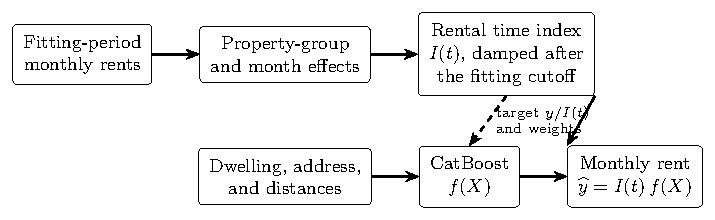
\includegraphics[width=0.96\linewidth]{model4_architecture.pdf}
\caption{Model~4: a global CatBoost with a property-adjusted
rental time index.
The dashed link supplies the index-based training target and weights.
Future monthly rents are restored using the forecast index.}
\label{fig:model4-architecture}
\end{figure}

\subsubsection{Performance}

Table~\ref{tab:model4-trials} compares the fixed-split experiments.
The local control does not exactly reproduce the original
recorded reference; that discrepancy is not an optimization gain.
Both are separate records from Model~3's 448.24/462.87 run above.

\begin{table}[htbp]
\centering
\caption{Sequential experiments on the fixed Search and Confirm periods.
Values are monthly-rent RMSE in SGD;Each row retains the preceding configuration and adds
the indicated modification..}
\label{tab:model4-trials}
\small
\setlength{\tabcolsep}{4pt}
\begin{tabularx}{\textwidth}{@{}Xrr@{}}
\toprule
Configuration & Validation & Test\\
\midrule
Global CatBoost (baseline)
& 447.78 & 455.21 \\
+ finer categorical statistics
& 445.38 & 452.87 \\
+ complete address
& 444.91 & 452.72 \\
\textbf{+ rental time index}
& \textbf{444.47} & \textbf{450.89} \\
\bottomrule
\end{tabularx}
\end{table}

The largest single-step reduction comes from the global
direct-rent model: 3.6776 on Search and 11.9000 on Confirm
relative to the local control.
Finer categorical statistics, complete address, and the time
index then provide further reductions.
These are sequential comparisons, not independent causal ablations.
The final model improves on the fixed local control by
6.9837 (1.55\%) on Search and 16.2182 (3.47\%) on Confirm.

The 50/50 blend has the lowest Search RMSE, but its Confirm
RMSE is worse than its global component's 452.8742,
so it was not retained.
Candidates failing their pre-specified Search gate were not
evaluated on Confirm.
The vacancy correction failed during historical calibration,
before either score was produced.
The final time-index candidate passed its Search threshold of
444.9107 before one Confirm evaluation.
Confirm had been inspected in earlier trials and is iterative
validation, not an untouched test set.

The frozen model produced 50{,}000 competition predictions
without refitting on all labelled rows.
The reported Kaggle RMSE is \textbf{441.46370}.
This is the latest submission already noted in the report.
It is the selected model with the lowest Confirm RMSE in this
series, but does not replace add\_mrt's 432.50 as the report's
best competition result.
Kaggle and local RMSEs score different data.
Search and Confirm cover forecast months 1--6; the historical
16/22-month checks assessed the index alone, so complete-model
long-horizon validation remains outstanding.

\FloatBarrier


\subsection{Comparison}
\label{sec:headline}

Table~\ref{tab:headline} separates local evaluation windows
from competition scores.
The local windows are not all the same cut of months.
Model~4's Search covers October--December 2024, while its
Confirm covers January--March 2025 and is iterative validation.
Model~1 scores October 2024 through March 2025 after a fit through September 2024.
Model~2 scores November 2023 through March 2025 after a fit through October 2023.
Model~3 scores October through December 2024 after a fit through September 2024, and that validation RMSE is the one that stops the model.

\begin{table}[htbp]
\centering
\caption{Comparison of monthly-rent RMSE, in SGD.
Local evaluation windows are defined separately above.
Model~4's Search and Confirm are named explicitly.
Competition scores are separate from all local evaluations.
The best private-test RMSE is 432.50, from add\_mrt.
The row 451.26 is an earlier private-test submission.}
\label{tab:headline}
\small
\setlength{\tabcolsep}{3pt}
\begin{tabularx}{\textwidth}{@{}>{\raggedright\arraybackslash}p{0.42\textwidth} X r@{}}
\toprule
Model & Window & RMSE \\
\midrule
Model 1, global mean & Validation set & 795.76 \\
Model 1, town mean & Validation set & 778.62 \\
Model 1, town + flat type & Validation set & 565.58 \\
Model 1, CatBoost & Validation set & 454.29 \\
Model 2, original + address & Validation set & 501.83 \\
Model 2, add\_mrt & Validation set & 499.53 \\
Model 2, all auxiliary, cutoff-frozen & Validation set & 517.51 \\
Model 2, all auxiliary, provided-lagged & Validation set & 553.50 \\
Model 3 & Validation set & 448.24 \\
Model 3 & Private test set & 451.26 \\
Model 2, add\_mrt & Private test set & 432.50 \\
Model 4 & Validation set & 444.47 \\
Model 4 & Private test set & 441.46 \\
\bottomrule
\end{tabularx}
\end{table}

On the validation set, Model~1's CatBoost RMSE is 454.29, against 795.76 for the global mean, 778.62 for the town mean, and 565.58 for the town and flat-type mean.
Model~2's add\_mrt validation RMSE is 499.53, a small improvement on original plus address at 501.83, while both all-auxiliary rows are higher.
Model~3's validation RMSE is 448.24, and that is the score that chose its epoch.
On the private test set, add\_mrt has RMSE 432.50.
That is the best private-test RMSE.
Gold Miner (Group 12) is rank 21 after eight submissions.
The latest submission scored a private-test RMSE of 441.46 and did not replace that best.
Model~3's earlier private-test submission scored 451.26.
A private-test RMSE is not the validation RMSE of another row, and it did not choose Model~3's epoch.

\subsection{Model 4}

\subsubsection{Temporal and Historical Rental Features}

Our experiments focused on improving HDB rental price prediction through temporal modelling and historical rental information. While property characteristics and location are important determinants of rent, rental prices also change over time and vary between individual housing blocks. We therefore investigated whether modelling market trends and incorporating previous rental transactions could improve the predictions of a CatBoost regression model.

\paragraph{Data Exploration and Preprocessing.}
The training dataset contains 150,000 rental records from January 2021 to March 2025, while the test set contains 50,000 records extending to July 2026. This creates a temporal prediction problem, since a substantial portion of the test data lies beyond the training period.

Our initial exploration showed that the average monthly rent increased from approximately S\$2,121 in 2021 to S\$3,036 in 2023, before reaching S\$3,110 in 2024. Although these averages are not adjusted for differences in the composition of rented flats, they suggest that the rental market experienced substantial changes over the training period, with slower growth in the later years.

We used HDB block information to obtain geographical and building-level attributes, including coordinates, planning areas and building age. We also calculated distances to nearby MRT stations, schools and shopping malls. Categorical variables such as town, block, street and flat type were retained for CatBoost, while additional numerical features were generated from property attributes and rental dates.

\paragraph{Baseline Model.}
We used CatBoost regression because the dataset contains a mixture of numerical and categorical variables. CatBoost can handle categorical features directly and has been shown to perform well on tabular datasets \cite{prokhorenkova2018catboost}.

The main experiments used a tree depth of 6, learning rate of 0.055, L2 regularisation of 5 and random seed 42. We initially compared different numbers of boosting iterations before fixing the model configuration for subsequent feature ablations.

\paragraph{Temporal Modelling.}
Our baseline already included year, month, quarter and a continuous time index. We investigated two additional temporal components.

First, we introduced cyclical month features:
\begin{equation}
    m_{\sin} = \sin\left(\frac{2\pi(m-1)}{12}\right),
    \quad
    m_{\cos} = \cos\left(\frac{2\pi(m-1)}{12}\right),
\end{equation}
where $m$ denotes the calendar month. These features were intended to capture possible annual patterns in rental demand.

Second, we constructed a monthly rental market index using historical log rents, adjusted for differences between town and flat-type groups. A recent trend was estimated from this index and extrapolated with exponential decay to avoid extending short-term growth indefinitely.

The final prediction was adjusted as
\begin{equation}
    \hat{y}_{i,t}
    =
    f_{\mathrm{CB}}(x_{i,t})
    \exp\left(\alpha\Delta_t\right),
\end{equation}
where $f_{\mathrm{CB}}$ is the CatBoost prediction, $\Delta_t$ is the estimated change in the rental market index and $\alpha$ controls the adjustment strength. We used $\alpha=0.5$ in the subsequent experiments.

\paragraph{Historical Rental Features.}
We further investigated whether previous rentals from the same HDB block could provide useful information beyond the geographical features already included in the model.

For each observation, we identified historical transactions sharing the same town, block, street and flat type. We then calculated the number of previous transactions, median rent, mean rent, standard deviation and the number of months since the most recent transaction.

To avoid target leakage, historical features were calculated using only transactions from strictly earlier months. During validation, only records available before the corresponding training cutoff were used as reference data. The current observation and transactions from the same or future months were excluded.

We subsequently tested additional street- and town-level statistics, recent rental windows of 3, 6 and 12 months, and nearby comparable rental transactions. These extensions allowed us to examine whether increasingly detailed historical information improved the model.


\subsubsection{Ablation Studies and Evaluation}

We evaluated our models using root mean squared error (RMSE), which is also the metric used in the Kaggle competition. We additionally examined mean absolute error (MAE) and prediction bias to better understand the models' behaviour.

Rather than using a random train-validation split, we adopted chronological validation. The three development validation periods were July--December 2023, January--June 2024 and July--December 2024. In each fold, the model was trained only on observations preceding the validation period. January--March 2025 was also examined separately as a diagnostic period.

The reported mean validation RMSE is the arithmetic average of the three development-fold RMSE values.

\paragraph{Temporal Feature Ablation.}
We first compared four configurations: the original CatBoost model (A), additional cyclical month features (B), market trend adjustment (C), and both modifications together (D). All models were evaluated using 1600 iterations.

\begin{table}[t]
\centering
\caption{Temporal feature ablation at 1600 iterations.}
\label{tab:temporal_ablation}
\small
\begin{tabular}{lcc}
\hline
Model & Mean RMSE & 2025 Q1 RMSE \\
\hline
A: Baseline & 519.60 & 450.39 \\
B: + Seasonality & 519.48 & 450.38 \\
C: + Market trend & 518.41 & 449.87 \\
D: + Both & \textbf{517.89} & \textbf{449.80} \\
\hline
\end{tabular}
\end{table}

As shown in Table~\ref{tab:temporal_ablation}, the market trend adjustment provided a more noticeable improvement than the cyclical month features. Adding seasonality alone produced only a small reduction in RMSE, possibly because the baseline already included month and quarter information.

The combined model achieved the lowest mean validation RMSE. However, the improvement over the baseline was relatively modest, suggesting that temporal modelling alone could not explain a large proportion of the remaining prediction errors.

\paragraph{Effect of Boosting Iterations.}
We also examined the effect of the number of boosting iterations. To separate the influence of training duration from feature engineering, we compared the original CatBoost model (A) and the combined temporal model (D) using 800, 1200, 1600 and 2000 iterations, while keeping other hyperparameters unchanged.

\begin{table}[t]
\centering
\caption{Mean validation RMSE across different boosting iterations.}
\label{tab:iteration_ablation}
\small
\begin{tabular}{rcc}
\hline
Iterations & Model A & Model D \\
\hline
800  & 520.17 & 518.51 \\
1200 & \textbf{519.60} & 517.95 \\
1600 & 519.60 & 517.89 \\
2000 & 519.74 & \textbf{517.88} \\
\hline
\end{tabular}
\end{table}

As shown in Table~\ref{tab:iteration_ablation}, increasing the number of iterations initially improved both models. However, the improvement became much smaller beyond 1200 iterations. For model D, increasing the iterations from 1600 to 2000 reduced the mean RMSE by only 0.01.

Although 2000 iterations achieved a marginally lower average RMSE, 1600 iterations performed slightly better on average in our additional long-horizon evaluation and required less training time. We therefore selected 1600 iterations for the subsequent historical feature experiments.

\paragraph{Historical Rental Feature Ablation.}
We next introduced historical rental features while keeping the CatBoost configuration fixed at 1600 iterations. Model F0 corresponds to model D from the temporal experiments.

\begin{table}[t]
\centering
\caption{Historical rental feature ablation.}
\label{tab:historical_ablation}
\small
\begin{tabular}{lcc}
\hline
Model & Mean RMSE & Difference vs. F0 \\
\hline
F0: Temporal baseline & 517.89 & -- \\
F1: + Block history & \textbf{514.83} & \textbf{-3.07} \\
F2: + Street/Town history & 519.01 & +1.12 \\
F3: + Recent rental windows & 528.70 & +10.80 \\
F4: + Nearby rentals & 535.78 & +17.89 \\
\hline
\end{tabular}
\end{table}

Table~\ref{tab:historical_ablation} shows that adding block-level historical rental features produced the largest improvement. F1 outperformed F0 in all four evaluated time periods. For example, its RMSE decreased from 460.22 to 455.98 in the second half of 2024, and from 449.80 to 444.29 in the first quarter of 2025.

Interestingly, adding more historical features did not necessarily improve performance. F2 was slightly worse than F0, while F3 and F4 showed substantial deterioration.

One possible explanation for F3 and F4 was that their recent rental windows became increasingly sparse when predicting further into the future. As the prediction horizon extended beyond the available training records, the model encountered historical features that differed from those observed during training.

We therefore conducted another experiment in which recent rental windows were fixed at the training cutoff, and additional time-normalised rental statistics were introduced. However, none of the revised configurations consistently outperformed F1. Their mean validation RMSE values ranged from 515.01 to 517.35, compared with 514.83 for F1.

These results suggest that local historical rental prices contain useful information, but adding more detailed statistics may introduce noise or unstable features.

\paragraph{Kaggle Evaluation.}
After selecting the model configuration through chronological validation, we retrained the final models using all 150,000 labelled training samples and generated predictions for the 50,000 test records.

Table~\ref{tab:kaggle_results} summarises the actual Kaggle Public Leaderboard results from successive submissions.

\begin{table}[t]
\centering
\caption{Kaggle Public Leaderboard results.}
\label{tab:kaggle_results}
\small
\begin{tabular}{lc}
\hline
Model & RMSE \\
\hline
Initial CatBoost & 441.78158 \\
D: Temporal model, 1200 iterations & 439.55517 \\
D: Temporal model, 1600 iterations & 438.28697 \\
F1: Block history, 1600 iterations & \textbf{432.50394} \\
\hline
\end{tabular}
\end{table}

The best submission was F1 with 1600 iterations, achieving an RMSE of 432.50394. This represents a reduction of approximately 9.28 RMSE, or 2.10\%, compared with our initial CatBoost submission.

In particular, adding block-level historical rental information improved the leaderboard RMSE from 438.28697 to 432.50394, while keeping the temporal modelling and CatBoost configuration unchanged.

The improvement is consistent with the chronological validation results, supporting the usefulness of local rental history for predicting individual HDB rents.


\subsubsection{Discussion and Limitations}

Our results indicate that historical rental information at the block level was more useful than increasingly complex temporal features. This is reasonable because two flats in the same town can still have different rental values depending on their exact location and building characteristics. Previous transactions from the same block provide a more local reference for estimating rental prices.

However, several limitations remain. First, historical transaction features depend on the availability of previous rentals. Blocks with limited rental history may have less reliable statistics. Second, the future rental market may differ from the training period, making long-term trend extrapolation difficult. The relatively limited benefit of the market trend adjustment suggests that a simple extrapolation of recent changes cannot fully represent future rental conditions.

The experiments with additional recent-window and neighbourhood statistics also demonstrated that more features do not always improve prediction accuracy. Some features may be noisy or poorly aligned with the information available at prediction time.

Finally, repeated evaluation on the Kaggle Public Leaderboard introduces a risk of overfitting model choices to the public test subset. The leaderboard results should therefore be interpreted together with chronological validation rather than as an unbiased estimate of generalisation performance.

Future work could investigate more robust historical rental statistics, particularly approaches that adjust previous rents for market changes while maintaining consistency between training and prediction. Further experiments with model ensembling and carefully selected additional features may also help reduce the remaining errors.

\FloatBarrier
\section{Limits and discussion}
\label{sec:limits}

The column limits in Section~\ref{sec:collimits} still apply to every model that uses those columns.
Great-circle distance is not walking time, opening dates are missing, and a group mean is a lagged rent rather than an attribute of the nearest school or station.
Furnished status and the fee do not vary.
They were removed from the core modelling table.
The fee name still occurs in the shared network's input list, and the value is 0 on every row, so that column carries no variation.

Scores from different windows do not rank the models.
The six-month hold-out RMSE of 454.29 and the computed multistage pool of 455.89 share the calendar months October 2024 through March 2025, and both fits can use months through September 2024.
They are still different procedures, and neither number is a private-test RMSE.
The multistage epoch was chosen on the validation set, October--December 2024, where the validation RMSE is 448.24.
The six-month hold-out RMSE is one evaluation of a fixed tree on all 17{,}198 rows.
The one-year hold-out RMSE of 477.47 fits only through March 2024 and scores a full year.
The 17-month add-MRT RMSE of 499.53 fits through October 2023.
A lower number on an easier or later cutoff is not evidence that one family dominates the other.
The best private-test RMSE is 432.50, from add\_mrt.
A private-test score is not comparable with a validation RMSE or a test RMSE as if they were the same split.
That private-test score did not choose Model~3's epoch.
An earlier private-test submission scored 451.26.
It is no longer the best and no longer the latest.
The latest submission scored a private-test RMSE of 441.46 and did not replace the best.

Inside the rebuilt CatBoost comparison, adding every auxiliary family did not lower the 17-month RMSE relative to original plus address.
Add-MRT did, by a small margin on that 17-month assessment, and it was the best predefined main CatBoost configuration on the development pooled RMSE.
The conditional distance screen is an association after controls.
It is not the selection rule, and the two secondary-school codings do not agree in sign.

The region mean uses a tanh hidden state, so it cannot grow without a bound.
On the private test set the multistage network's cross-town unit-price mean stays near 35.99 in April 2025 and 35.79 in July 2026.
A linear bypass can keep a slope past the training set.
The comparisons that were run still favoured the recurrent network.
On the dollar town-month mean, the linear bypass had validation cell RMSE 170.56.
A one-layer dollar recurrent network, whose cross-town mean moved from 3192 in April 2025 to 3274 in July 2026, stayed closest to an external approved-rent path of about 3179 to 3280.
Those public rents were an external check only.
They were not training labels.
On the per-square-metre target, a linear-bypass LSTM had validation cell RMSE 1.9646 and test cell RMSE 3.4044, against validation cell RMSE 0.9707 and test cell RMSE 1.0897 for the three-layer network in the stack.
Dollar cell RMSEs and per-square-metre cell RMSEs are different targets.
Appendix~\ref{app:dollar} keeps them in separate tables.

The training-set rent RMSE of 461.25 uses the town CatBoost's predictions on its own training rows.
The validation features of that CatBoost come from a model whose iteration was stopped on the validation set.
The test RMSE of 462.87 is the labelled score after the choice.
An earlier correlation of 0.890, with mean absolute error 69.1 across 76 components, is a dollar location check.
It was not recomputed on the five-dimensional per-square-metre mixture.
The Bukit Panjang figure was not scored.
The best private-test RMSE of 432.50 did not choose the epoch, the mixture, or the region network.

\FloatBarrier
\section{Conclusion}
\label{sec:conclusion}

The core audit supports a chronological split.
On its validation set, Model~1's CatBoost reaches RMSE 454.29, against 795.76 for the global mean, 778.62 for the town mean, and 565.58 for the town and flat-type mean.
Among the rebuilt CatBoost configurations, add\_mrt is the best.
Its validation RMSE is 499.53, and using every auxiliary family is higher than original plus address.

The best private-test submission is add\_mrt.
Its private-test RMSE is 432.50.
Gold Miner (Group 12) is rank 21 after eight submissions.
The latest submission scored a private-test RMSE of 441.46 and did not replace that best.
An earlier private-test submission scored 451.26.
It is no longer the best and no longer the latest.
The private-test score did not stop or choose Model~3.
Figure~\ref{fig:kaggle} is that private test set.

Model~3 remains the multistage stack.
A per-town recurrent network estimates the town-month rent per square metre from the time index and the economic trend already observed before the month being predicted.
A per-town CatBoost and a per-town Gaussian mixture estimate the unit-price gap separately.
One shared network turns the mean, both gaps, floor area, and the flat's other features into monthly rent.
The validation set selected epoch 8, with validation RMSE 448.24.
The test RMSE is 462.87 and did not make that choice.
Training RMSE on the training set is 461.25.

Model~4 pools all towns in one CatBoost and combines complete-address
encoding with a property-adjusted rental time index.
It reaches Search RMSE 444.47 and Confirm RMSE 450.89,
reducing error by 1.55\% and 3.47\% against its fixed local control.
Its frozen submission scores 441.46370 on Kaggle.
These results support the selected local optimization,
while add\_mrt remains the best competition submission in this report.

\begin{figure}[htbp]
\centering
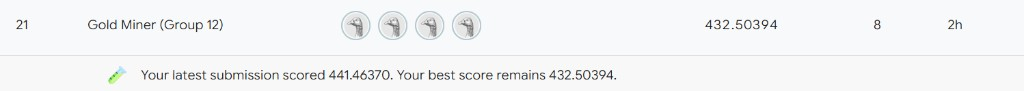
\includegraphics[width=0.98\linewidth]{kaggle_leaderboard.png}
\caption{Private test set, Gold Miner (Group 12), rank 21, eight submissions, best private-test RMSE 432.50.
The latest submission scored a private-test RMSE of 441.46 and did not replace that best.}
\label{fig:kaggle}
\end{figure}

\appendix
\section{Core CatBoost settings and the cyclical month}
\label{app:cyclic}

The core CatBoost in Section~\ref{sec:core-model} uses 600 boosting iterations, learning rate 0.05, depth 8, and random seed 42.
Categorical fields are supplied directly.
The cyclical check adds
\[
\sin\Bigl(2\pi\frac{m-1}{12}\Bigr)
\quad\text{and}\quad
\cos\Bigl(2\pi\frac{m-1}{12}\Bigr),
\]
where \(m\) is the calendar month, on top of the year, the numerical month, and the month index.
Table~\ref{tab:cyclic} is the three rolling folds.
A positive change is an increase in rolling-fold RMSE.
The pair is not kept.

\begin{table}[htbp]
\centering
\caption{Sine and cosine of calendar month, added to the core CatBoost on the rolling folds.
Positive change means a higher rolling-fold RMSE.
The mean row averages the three rolling-fold RMSEs.}
\label{tab:cyclic}
\small
\begin{tabular}{lrrr}
\toprule
Fold & Existing time features & Plus cyclical month & Change \\
\midrule
1 & 719.52 & 729.00 & $+9.49$ \\
2 & 599.59 & 610.34 & $+10.75$ \\
3 & 477.47 & 477.83 & $+0.36$ \\
\midrule
Mean & 598.86 & 605.73 & $+6.87$ \\
\bottomrule
\end{tabular}
\end{table}

\section{Dollar town-month trials}
\label{app:dollar}

The recurrent network in the stack is trained for 50 epochs at learning rate 0.01 with seed 5228, on cells in the training set.
The trials in Table~\ref{tab:dollar} predict the town-month mean of monthly rent, in SGD.
They are not the per-square-metre target.
The one-layer dollar network's private-test cross-town mean moves from 3192 in April 2025 to 3274 in July 2026, closest among these dollar paths to the external approved-rent path of about 3179 to 3280.
That external path was a check, not a training label.
The four-input three-layer LSTM moves from 3132 to 3109.
The linear bypass beside that LSTM fits the training cells, with training-set cell RMSE 83.73, and then overshoots: validation cell RMSE 170.56, test cell RMSE 261.29, and a private-test path from 3339 to 3821.

\begin{table}[htbp]
\centering
\caption{Dollar town-month mean of monthly rent.
Cell RMSE is in SGD.
These numbers are not comparable with Table~\ref{tab:unit}.}
\label{tab:dollar}
\small
\begin{tabular}{lrr}
\toprule
Model & Validation cell RMSE & Test cell RMSE \\
\midrule
One-layer recurrent network & 93.25 & 88.04 \\
Four-input, three-layer LSTM & 88.75 & 83.39 \\
Linear bypass beside that LSTM & 170.56 & 261.29 \\
\bottomrule
\end{tabular}
\end{table}

Table~\ref{tab:unit} is the per-square-metre target.
The three-layer recurrent network is the region mean in the multistage stack.
Its cross-town unit mean on the private test set goes from 35.99 in April 2025 to 35.79 in July 2026.
The test-set per-square-metre cell RMSE did not choose the network.

\begin{table}[htbp]
\centering
\caption{Town-month mean of rent per square metre.
Cell RMSE is in SGD per square metre, weighted by the number of flats in the cell.
These numbers are not comparable with Table~\ref{tab:dollar}.}
\label{tab:unit}
\small
\begin{tabular}{lrr}
\toprule
Model & Validation cell RMSE & Test cell RMSE \\
\midrule
Three-layer recurrent network & 0.9707 & 1.0897 \\
Linear-bypass LSTM & 1.9646 & 3.4044 \\
\bottomrule
\end{tabular}
\end{table}

A wider perceptron, with widths 512, 256, 128, and 64, dropout 0.3, and patience 40, was tried on an earlier dollar region mean.
Its validation RMSE of monthly rent was 448.88 and its test RMSE was 461.87 at epoch 29.
That validation RMSE belongs to a different region mean.
It is not a comparison with the stack's validation RMSE of 448.24, and it is not the stack prediction.

\section{Gap models and the shared network}
\label{app:gap}

The town CatBoost uses depth 8, learning rate 0.05, at most 1000 iterations, and early stopping of 50 rounds on the validation set.
Its columns are latitude and longitude; the block key and the street key; flat-type rank, flat-model rank, and flat-model name; nearest open MRT code, distance, and log distance; nearest mall name and distance; and nearest primary and secondary names and distances.
Categories stay native.
Numeric columns are median-imputed and are not scaled.
A rare level needs 30 rows.
An unseen category becomes a missing token.
This list is not the feature set produced by the column-by-column ablation in Appendix~\ref{app:ablation}.
That ablation does not choose the town stage, and the stack does not replace it.

Each town's mixture starts at 20 components.
If any component that is hard-assigned on the training set has fewer than 30 rows, the count drops by one and the town is refit, down to one component.
Bukit Panjang kept 6.
Across towns the kept counts in the scored training run from 3 to 19.

An earlier location check, on a dollar gap rather than this five-dimensional unit-price mixture, is a separate result.
Across 76 components, the training-set dollar gap and the validation-set gap correlate 0.890, with mean absolute error 69.1.
An own-town surface starting at three components has validation RMSE 578.11 and test RMSE 593.19.
A density blend across towns has validation RMSE 579.76 and test RMSE 594.42.
Starting the own-town surface at 10, with the same drop rule, has validation RMSE 566.55 and test RMSE 580.58.
That correlation was not recomputed for the per-square-metre mixture in the stack.
The multistage mixture's flat-level validation RMSE and test RMSE are in Table~\ref{tab:gap}.

The shared network is optimised with Adam, learning rate 0.001, and batch size 1024.
The target is monthly rent, standardized on the training set and restored before the error is computed.
The 27 inputs are the recurrent-network unit mean, the CatBoost unit gap, the mixture unit gap, and floor area; the fee, which is 0 on every labelled row and every private-test row and so does not vary; lease commencement year; building age; month index; latitude and longitude after within-town standardization; raw latitude and longitude in degrees; flat-type rank; flat-model rank; maximum floor; year completed; flat age from the lease; distances to the nearest open MRT station, mall, primary school, and secondary school; the log MRT distance; counts of open MRT stations, malls, primary schools, and secondary schools within 1\,km; and the count of other HDB blocks within 500\,m.
Furnished status is not an input.

\section{Feature ablation}
\label{app:ablation}

The ablation adds auxiliary columns one at a time.
It starts from a model already fit on the ten source columns.
Architecture and preprocessing stay fixed.
Only the validation RMSE decides whether a column is kept.
The test RMSE is recorded after that decision and does not enter it.

Set A is the column list saved at the start of a round.
Each auxiliary column that is not already in set A is tried on its own.
That probe is set B, equal to set A plus the one new column, trained with the same budget as set A.
A probe does not replace the saved list.
For ridge and the multilayer perceptron, the column is promising only when the probe's validation RMSE is at least 1\% below set A's validation RMSE.
For XGBoost and CatBoost, the column is promising when the probe's validation RMSE is strictly lower.
Set C is set A plus every promising column from that round, trained once.
Set C replaces the saved list only when its own validation RMSE is lower than set A's.
The next round then treats that new list as set A.
The loop stops when a round has no promising column, or when set C does not win.
A later retraining uses only the columns already kept, with a larger budget, and does not add or drop columns.

\end{document}
